\documentclass[a4paper,12pt,%
headsepline,%
numbers=noenddot,% entfernt die Punkte nach den Gliederungsziffern
]{scrreprt}

\usepackage[T1]{fontenc}
\usepackage[utf8]{inputenc}
\usepackage[ngerman]{babel}
\usepackage{setspace} 

%-----------Format-------------
%\usepackage{titlesec} %Titel Format bearbeiten
\usepackage{setspace} 
\setstretch{1,15} % 1,5 Zeilenabstand, [singlespacing] oder [doublespacing] auch möglich
\usepackage{lscape} % für Querformat

%-----------hübsche Darstellung -------------
\usepackage[per=slash,decimalsymbol=comma,loctolang=ngerman]{siunitx} % SI-Einheiten werden schick dargestellt
\sisetup{locale = DE} % Komma als Trenner bei Dezimalzahl erkannt
\sisetup{detect-all} %SI-Einheiten in "normaler" Schriftart


%-----------Grafiken und Tabellen-------------
\usepackage{float} %float-Objekte mit Großbuchstaben an Stelle behalten
\usepackage{caption} % Beschriftungen von Bildern & Tabellen bearbeiten
\captionsetup{format=plain,
	font=small,
	width=0.95\textwidth,
	labelfont=bf}
\captionsetup[table]{singlelinecheck=false,
	name=Tab.}
\captionsetup[figure]{name=Abb.}

\usepackage{graphicx} % Grafiken einbinden

\usepackage{booktabs} % Tabellen ordentlich, toprule, midrule, cmidrule, bottomrule
\usepackage{tabularx} % Tabelle eine bestimmte Breite vorgeben, automatischen Zeilenumbruch innerhalb der Spalten
\usepackage{threeparttable} % Beschriftung von Tabellen auf Tabellenbreite, Fußnoten an Tabellen uvm; muss um die tabular Umgebung herum gesetzt werden
\usepackage{multirow} % erlaubt es, Zeilen bzw. Spalten miteinander zu verschmelzen
\usepackage[table,xcdraw]{xcolor} % farbige Zellen

%-----------Listen-------------
\usepackage{outlines} %Verschachtelte Listen deutlich einfacher
\usepackage{enumitem} %Anpassbare Enumerates/Itemizes, Listen global konfigurieren
\setitemize{nosep} %Abstand zwischen Items, verwende auch itemsep=0p


%-----------weiterer Komfort-------------
\usepackage{textgreek} %Griechische Buchstaben mit \textalpha etc.
\usepackage{tikz} % Zeitstrahl
%\usetikzlibrary{snakes}
\usepackage{chronosys}


%----------überprüfen------------
\usepackage{microtype}

%----------zuletzt laden---------
\usepackage[%pdflatex,%
pagebackref=true,%
pdfauthor={Ink Inc.},%
pdftitle={Wissenssammlung},%
pdfsubject={Handbuch}%
]{hyperref} %







%----------eigene Befehle--------
\newcommand{\npref}[1]{\nameref{#1} (S. \pageref{#1})} 
% Überschriften
% wenn \npref{referenz} aufgerufen wird, wird automatisch eine Sequenz eingefügt: "`Name (s. X)"' zB "`Sylvan (S. 3)"'
\newcommand{\epref}[1]{\ref{#1} (S. \pageref{#1})} 
% Tabellen und Abbildungen
% wenn \epref{referenz} aufgerufen wird, wird automatisch eine Sequenz eingefügt: "`Zahl (s. X)"' zB "`3.5 (S. 3)"'
\newcommand{\zB}{z.~B.} %automatisches Ersetzen von zB

%----------Vorlagen--------
%Tabelle
%\begin{table}[htb]
%	\centering
%	\caption[Knapper Titel]{Sehr informativer Titel}
%	\label{tab:key}
%	\begin{threeparttable}
%		\begin{tabularx}{\textwidth}{l|ccX} %wenn die Tabelle eh schmaler als die Textbreite ist und eine rein vom Inhalt dynamische Breite gewünscht ist, muss hier und unten das x hinter tabularx sowie die zweite geschweifte Klammer entfernt werden!
%			\toprule
%			\textbf{1st Column} & \textbf{2nd Column} & \textbf{3rd Column} & \textbf{4th Column} \\ 
%			\midrule
%			QWERTY\tnote{1}   &                     &                     &  \\
%			ASDFGH   &                     &                     &  \\ 
%			\bottomrule
%		\end{tabularx}
%		\begin{tablenotes}
%			\item[1] qwerty
%		\end{tablenotes}
%	\end{threeparttable}
%\end{table}

%  Aufzählung (1.,2.,...)
%\begin{enumerate}
%	\item 
%\end{enumerate}

% Liste mit Symbolen
%\begin{outline}
%	\1 This is a first item.
%	\1[!!!] This is a second, with a custom label.
%		\2 A level-2 item.
%			\3 A level 3.
%				\4 Deepest is level 4.\
%		2 Back to level 2.
%\0 A normal paragraph in the middle.\
%	1 A couple more
%		\2 items.
%\end{outline}

% Gedankenstrich durch: --

\begin{document}

\begin{titlepage}
	\centering
	\vfill
	\Large{\textbf{Stand {\today}}} \\ \bigskip
	\vfill
	\textsf{\textbf{\Huge{Wissenssammlung}}} \\ \bigskip
	\Large{\textbf{zur Übersicht der Geschichte von MMG der Ink Inc.}} \\ \bigskip
	\vfill
	\includegraphics[width=\linewidth]{Abbildungen/logo.png} \\ \bigskip
	\vfill
	\large
	bearbeitet von\\
	Medsmiley, Thabb, Mine Schokokeks, MiMi, LuckerStyle, Dommmmmi, Liandarin \\ \bigskip
	Bilder von Fossor, Kriluny, Liandarin
\end{titlepage}

\pagenumbering{Roman}
\tableofcontents
\listoffigures



%----------Inhalt-------------
\chapter*{Einleitung}
\pagenumbering{arabic}
Dieses Dokument dient zur Sammlung und Aufbewahrung allen beschlossenen Wissens bezüglich des MMG Spiels der Ink Inc. 
Die Lore soll einen guten Hintergrund geben, damit eine Vorstellung der Welt existiert. 
Damit lässt sich dann die Gesellschaft aufbauen, in der der Spieler seinen Charakter das Abenteuer erleben lässt. \\

Nichts zu suchen haben hier detaillierte NSC- oder Questbeschreibungen. 
Dieses Netzwerk aus Beziehungen erfassen wir in einer eigens dafür erstellten Plattform. 
Die Mechaniken wiederum finden sich in der gleichnamigen PDF.

\part{Weltenbau}
\chapter{Karte \& Ökologie}
\section{Sonnensystem}
\href{http://www.weltenbau-wissen.de/sci-fi-erschaffen-fantasy-welt-erstellen-einstieg/}{Welt erstellen} \\
\href{http://www.weltenbau-wissen.de/2015/10/weltenbau-fragenkatalog-oekologie-biologie/}{Fragenkatalog} \\
\href{http://www.weltenbau-wissen.de/2015/01/weltenbau-mit-weltkarte-karte-zeichnen-tutorial/}{Weltkarte zeichnen} \\
\href{https://inkarnate.com/}{Weltenbautool}

\paragraph{Hintergedanke}
Das Ziel war es, ein System zu schaffen, welches uns erlaubt, so nahe wie möglich an den Gegebenheiten unserer Erde anzusetzen.
Dadurch wird erzielt, dass nur weniges geändert werden muss und der Großteil eins zu eins übernommen werden kann.
Besteht jedoch der Wunsch nach Änderung, so ist er immer möglich.
Im Sinne der Mystik wurde ein Planetensystem geschaffen, das ganz anders ist als unseres -- und doch ähnliche Bedingungen wie auf der Erde erlaubt.
Dazu mehr im entsprechenden Abschnitt.




\section{Planetensystem}
Wie in Abb. \ref{fig:planeten-system} zu sehen, gibt es zwei sich umkreisende Planeten, Andar und Gara, und ihren Mond Serro.
Andar und Gara drehen sich auf der gleichen Ebene um einen gemeinsamen Mittelpunkt, weshalb sie am Himmel des jeweils anderen immer an der gleichen Stelle stehen.
Dabei hat sich ihre Eigenrotation aneinander angeglichen, wodurch sie sich permanent mit der gleichen Seite ansehen (wie auch der Mond die Erde).

Damit es auch Ebbe und Flut geben kann, wird der gemeinsame Mittelpunkt von Serro auf der senkrechten Achse zur Planetenebene umkreist. 
Allerdings hält er dabei immer den gleichen Abstand zu beiden Planeten -- er hat also gleichzeitig auch die gemeinsame Bewegung auf der Planetenebene, damit dies möglich ist.

Dieses gesamte Gebilde, verdeutlicht in Abb. \ref{fig:planeten-konzept}, ist auf seiner elliptischen Sonnen-Umlaufbahn um 23 Grad gekippt, zugunsten der Existenz von Jahreszeiten.
Serro fungiert auch als Asteroidenfänger.
Somit sind die Innenseiten der Planeten schon immer verschont geblieben, allerdings ihre Außenseiten nicht.
Dort ist ab und an Gestein aus dem All eingeschlagen, weshalb die äußeren Seiten auch diverse Krater aufweisen und weniger besiedelt sind, als die Inneren.

\begin{figure}[tbh]
	\centering
	\includegraphics[width=0.9\linewidth]{Abbildungen/Weltenbau/Welt/planeten-system}
	\caption[Das Planetensystem]{\textbf{Das Planetensystem.}\\
	Die Planeten Gara (v.l.) und Andar (v.r.) mit ihrem Mond Serro (h.).}
	\label{fig:planeten-system}
\end{figure}

\begin{figure}[tbh]
	\centering
	\includegraphics[width=0.9\linewidth]{Abbildungen/Weltenbau/Welt/planeten-konzept}
	\caption[Konzept des Planetensystems]{\textbf{Darstellung der Rotationsachsen des Planetensystems.}\\
	Es ist de Neigung zur Umlaufbahn um die Sonne zu sehen, als auch die Linien, auf denen sich die drei Bestandteile des Systems drehen.}
	\label{fig:planeten-konzept}
\end{figure}

\paragraph{Entstehung des Systems} 
Ähnlich zu der Entstehung von Erde und Mond sind auch Andar, Gara und Serro aus einem größeren Brocken entstanden.
Während er noch frisch und recht flüssig war, traf ihn ein anderer großer Brocken und so spalteten sie sich in drei Klumpen auf, die sich in eine stabile Rotation umeinander einfanden.
Annähernde Daten zu den Dreien finden sich in Tab. \ref{tab:planetendaten}.

%TODO diese Tabelle wird nicht kompiliert
%\begin{table}[htb]
%	\centering
%	\caption{\textbf{Eckdaten des Planetensystems.}}
%	\label{tab:planetendaten}
%	\begin{threeparttable}[\linewidth]
%		\begin{tabular}{l|cc}
%			\toprule
%			\textbf{Größe} & \textbf{Wert in SI-Einheiten} & \textbf{Wert in natürlichen Größen}\\
%		    \midrule
%		    Masse der Sonne $M_S$ & $2,63\cdot 10^{30}$ kg & $1,3\,M_\odot$\\
%		    Leuchtkraft der Sonne $L_S$ & $1,17\cdot 10^{27}$ W & $3,06\,L_\odot$\\
%		    Temperatur der Sonne $\Theta_S$ & $5.778$ K & $1\,\Theta_\odot$\\
%		    Radius der Sonne $R_S$ & $780.093$ km & $1,12\,R_\odot$\\
%		    Sehwinkel der Sonne $\alpha_S$ & $0,34$° & $0,64\,\alpha_\odot$\\
%		    Absolute Helligkeit der Sonne $M^{bol}_S$ & $3,527$ & $0,73\,M^{bol}_\odot$\\
%		    Scheinbare Helligkeit der Sonne $m_S$ & $-26,83$ & $1,003\,m_\odot$\\
%		    Distanz zur Sonne $d_S$ & $2,62\cdot 10^8$ km & $1,749$ AU\\
%		    Jahresdauer $T_S$ & $420\,d = 336\,T_P$ & $1,15\,yr$\\
%		    Neigung der Planetenachse & $23$° & $0,98\cdot 23,5$°\\
%		    Masse beider Planeten $M_P$ & $5,972\cdot 10^{24}$ kg & $1\,M_\oplus$\\
%		    Dichte der Planeten $\rho_P$ & $5,51\,\frac{g}{cm^3}$ & $1\,\rho_\oplus$\\
%		    Radius der Planeten $\R_P$ & $6.372$ km & $1\,R_\oplus$\\
%		    Tagesdauer $T_P$ & $30$ h & $1,25$ d\\
%		    Monatsdauer (12 Monate) & $28\,T_P$ & $35$ d\\
%		    Abstand der Planeten $d_P$ & $49.785$ km & -\\
%		    Sehwinkel Gara vom Äquator $\alpha_{P,E}$ & $16,90$° & -\\
%		    Sehwinkel Gara von den Polen $\alpha_{P,P}$ & $14,60$° & -\\
%		    Masse des Mondes $M_M$ & $2,854\cdot 10^{23}$ kg & $3,884\,M_\bullet$\\
%		    Dichte des Mondes $\rho_M$ & $3,34\,\frac{g}{cm^3}$ & $1\,\rho_\bullet$\\
%		    Radius des Mondes $R_M$ & $2.728$ km & $1,57\,R_\bullet$\\
%		    Distanz Mond-Planet $d_M$ & $49.785$ km & $0,13\,d_\bullet$\\
%		    Mondumlaufzeit $T_M$ & $17,5$ h & $0,03\,T_\bullet$\\
%		    Sehwinkel Mond am Äquator $\alpha_{M,E}$ & $6,67$° & $\sim 750\,\alpha_\bullet$\\
%		    Sehwinkel Mond bei $30$° $\alpha_{M,30}$ & $7,21$° & $\sim 811\,\alpha_\bullet$\\
%		    Fallbeschleunigung Punkt 1 $g_1$ & $9,56\,\frac{m}{s^2}$ & $0,97\,g_\oplus$\\
%		    Fallbeschleunigung Punkt 2 $g_2$ & $9,70\,\frac{m}{s^2}$ & $0,99\,g_\oplus$\\
%		    Fallbeschleunigung Punkt 3 $g_3$ & $9,91\,\frac{m}{s^2}$ & $1,01\,g_\oplus$\\
%		    Fallbeschleunigung Punkt 4 $g_4$ & $9,96\,\frac{m}{s^2}$ & $1,02\,g_\oplus$
%			\bottomrule
%		\end{tabular}
%	\end{threeparttable}
%\end{table}

Kommentare zu den Angaben:
\begin{outline}
	\1 Die Symbole $\odot$, $\oplus$ und $\bullet$ stehen für unsere Sonne, unsere Erde und unseren Mond.
	\1 Die Relationen sind in den Grafiken \ref{fig:planetensystem-fern}, \ref{fig:planetensystem-nah} und \ref{fig:planetensystem-positionen} skizziert. Letztere zeigt auch die Position der 4 berechneten Punkte für die Messung der Fallbeschleunigung.
	\1 Die Daten der Sonne sind so gewählt, dass die scheinbare Helligkeit und Strahlungsleistung auf Andar wie auf der Erde sind und die Sonne die gleiche Farbe hat wie unsere Sonne.
	\1 Der Abstand des Planetensystems von der Sonne ist so gewählt, dass die Planeten in der habitablen Zone der Sonne liegen und das Jahr 336 Andar-Tage (420 Erden-Tage) hat, welche sich schön in 12 Monate mit je 28 Tagen aufteilen lassen. Durch dubiose Resonanzen oder göttliche Fügung sind die ganzen Zahlen exakt, sodass es keine Schaltjahre oder ähnliche seltsame Phänomene gibt.
	\1 Die beiden Planeten vollführen eine doppelt gebundene Rotation (beide schauen sich die ganze Zeit mit der gleichen Seite an) und rotieren einmal pro Tag umeinander (30h). Die Rotationsebene der beiden Planeten ist gerade ausreichend geneigt, dass Gara nie die Sonne verdeckt und man klare Tag-Nacht-Zyklen definieren kann. Die gebundene Rotation sorgt dafür, dass die Rotationsachsen der einzelnen Planeten (Pole) senkrecht zur Verbindungsline zwischen den Planeten liegt.
	\1 Die doppelt gebundene Rotation führt außerdem dazu, dass immer die gleichen Hemisphären der Planeten außen liegen und diese stark von Meteoriteneinschlägen betroffen sind. Daher ist nur eine Hälfte der beiden Planeten gut bewohnbar. Meteoriten, die auf die inneren Hemisphären treffen könnten, werden zum Großteil vom Mond abgefangen.
	\1 Die Planeten an sich sind so gewählt, dass sie die gleichen Eigenschaften wie die Erde haben und damit eine stabile Atmosphäre halten und Leben beherbergen können.
	\1 Der Abstand der Planeten ist so gewählt, dass der Tag auf Andar (oder auch Gara) 30 h lang ist, da viel sich vermutlich negativ auf die Entwicklung von intelligentem Leben ausgewirkt hätte.
	\1 Der Mond kreist um die Verbindungsachse zwischen den beiden Planeten und steht zu allen Zeiten im dritten Punkt eines gleichseitigen Dreiecks mit diesen. Dieser Punkt gewährt eine erhöhte Stabilität des Systems (vgl. Lagrange-Punkte 4/5). Das hat zur Folge, dass der Mond sehr nah an den Planeten ist und eine sehr kurze Umlaufzeit hat, er umkreist die Planeten innerhalb von 7 Tagen 12 mal. Da nur die nach innen gerichteten Hälften der Planeten von Interesse sind, ignorieren wir die anderen Seiten. Die Flut verläuft dann auf einem Kreis mit 60° Neigung zur Verbindungsachse zwischen den Planeten und hat wegen des Mondes eine Periodendauer von 14h. Zudem ist aufgrund der Nähe des Mondes zu den Planeten die Flut um einiges stärker als auf der Erde.
	\1 Aufgrund der geringen Entfernung der beiden Planeten ist die scheinbare Größe von Gara am Himmel recht verschieden je nachdem, wo man sich auf Andar befindet. Ähnlich verhält es sich mit dem Mond, wobei dort die absoluten Unterschiede geringer sind, das dieser kleiner ist.
	\1 Ebenfalls eine Folge des geringen Abstandes ist die vergleichsweise starke Schwankung der Fallbeschleunigung auf der Oberfläche von Andar. In der Nähe der Verbindungslinie zu Gara ist die Anziehungskraft von Gara nach oben gerichtet, sodass die Fallbeschleunigung etwas geringer ist als auf der Erde. Auf der gegenüberliegenden Seite tritt dieser Effekt gerade umgekehrt auf. Auch der Winkel und Abstand zum Mond sowie der Winkel zu den Polen haben einen, wenn auch geringen, Einfluss auf die Fallbeschleunigung und führen zu weiteren Variationen. Effektiv zeigen wird sich das vermutlich kaum, da die relativen Unterschiede nur wenige Prozent betragen und wir uns sowieso nur auf einer Halbkugel von Andar befinden.
\end{outline}

\begin{figure}[tbh]
	\centering
	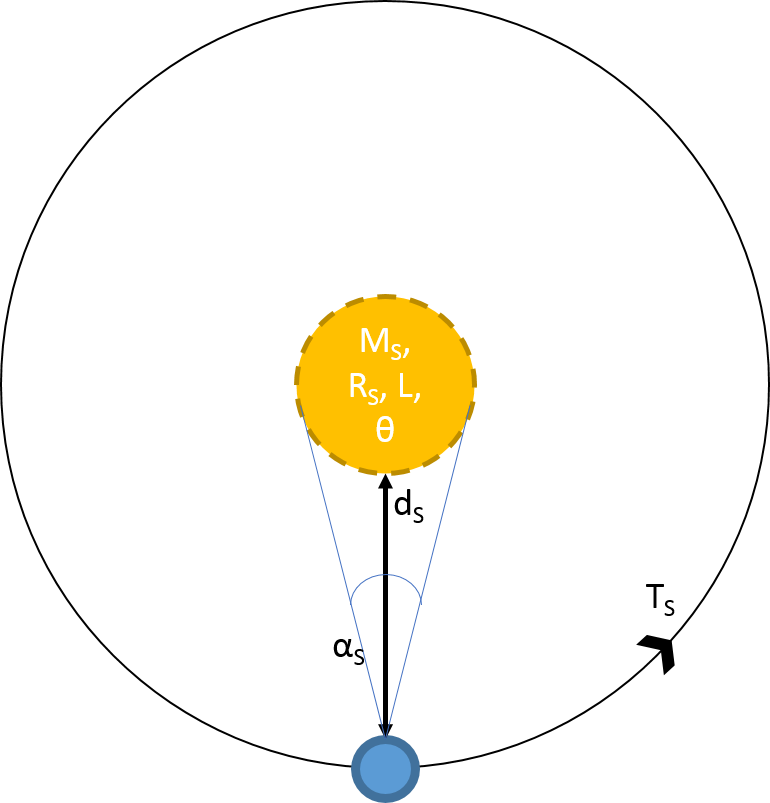
\includegraphics[width=0.9\linewidth]{Abbildungen/Weltenbau/Welt/planetensystem-fern}
	\caption[Planetensystem Skizzen 1]{\textbf{Das Planetensystem aus der Draufsicht auf die planetare Ebene.}\\
	Die Sonne (gelb) und das System der beiden Planeten einschließlich Mondes (blau).}
	\label{fig:planetensystem-nah}
\end{figure}

\begin{figure}[tbh]
	\centering
	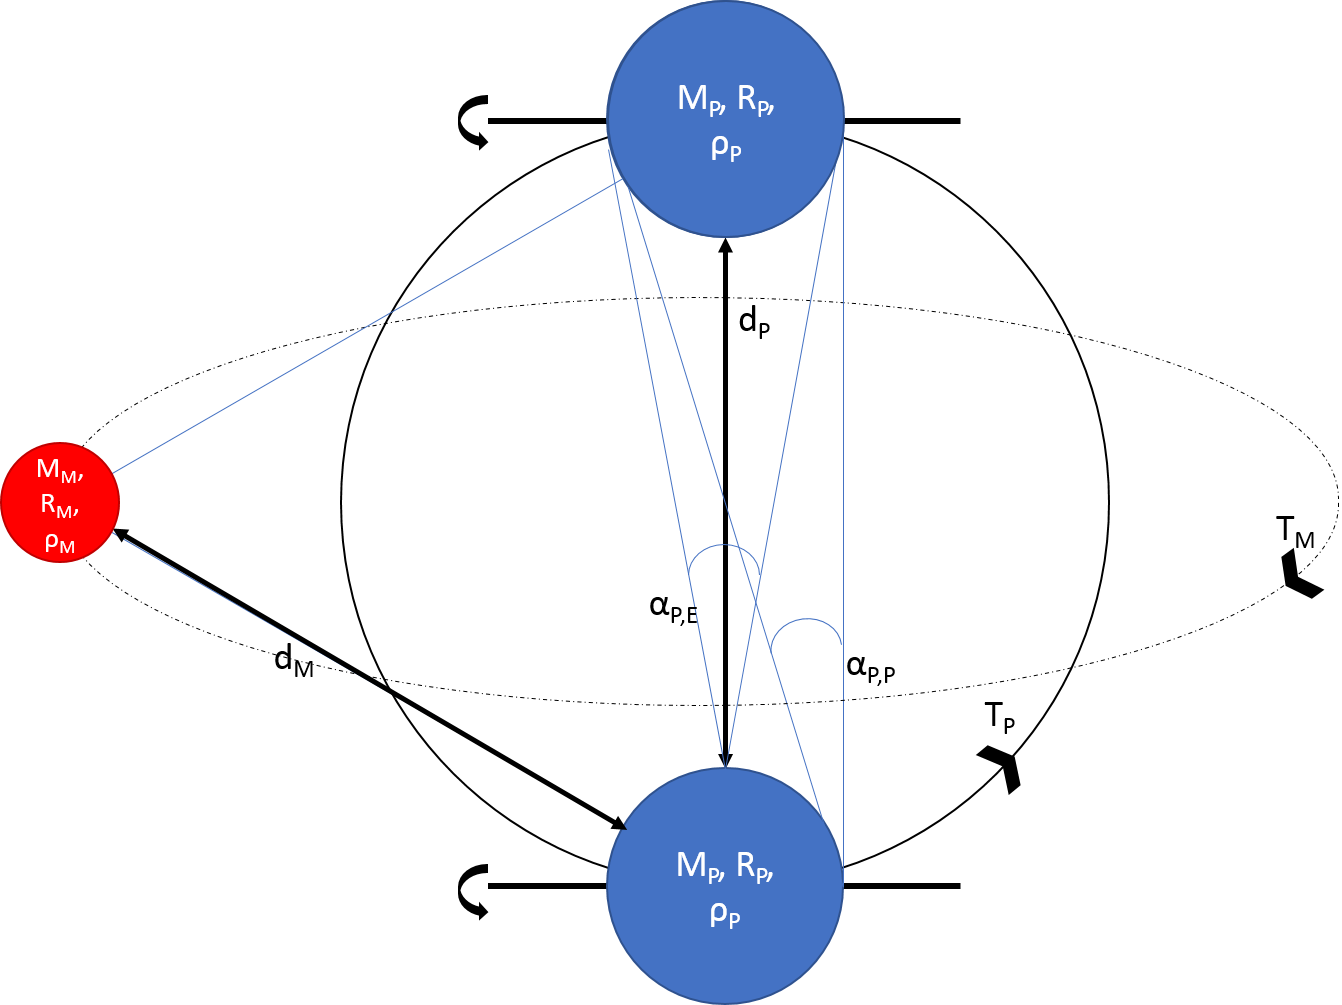
\includegraphics[width=0.9\linewidth]{Abbildungen/Weltenbau/Welt/planetensystem-nah}
	\caption[Planetensystem Skizzen 2]{\textbf{Das Planetensystem auf der Draufsicht auf die gemeinsame Ebene von Mond und Planeten.}\\
	Die Planeten Gara (o.) und Andar (u.) mit ihrem Mond Serro (l.).}
	\label{fig:planetensystem-fern}
\end{figure}

\begin{figure}[tbh]
	\centering
	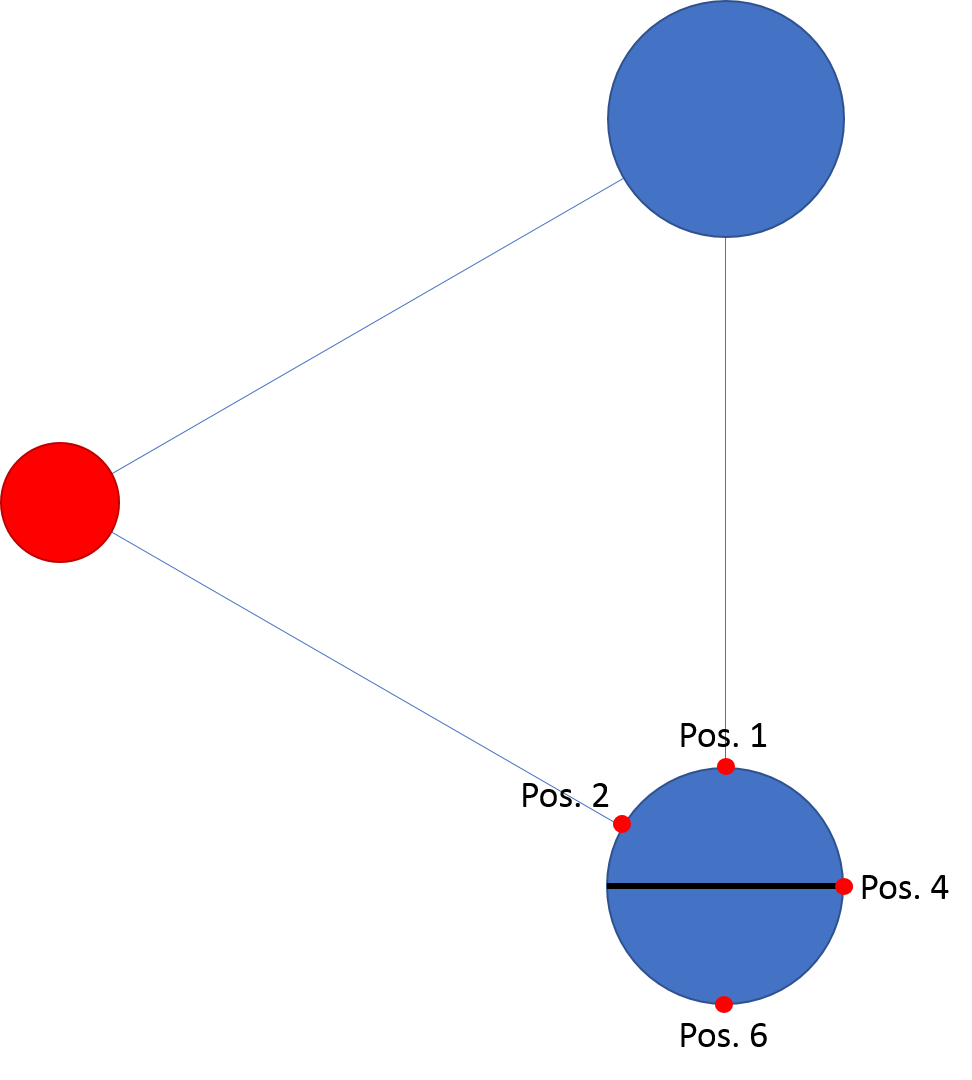
\includegraphics[width=0.9\linewidth]{Abbildungen/Weltenbau/Welt/planetensystem-positionen}
	\caption[Planetensystem Skizzen 3]{\textbf{Positionen für Messung der Fallbeschleunigung.}\\
	Die Planeten Gara (o.) und Andar (u.) mit ihrem Mond Serro (l.). Rote Punkte indizieren die berechneten Stellen für die Fallbeschleunigung.}
	\label{fig:planetensystem-positionen}
\end{figure}

\paragraph{Entstehung von Leben}
Das Leben entwickelte sich auf beiden Planeten unabhängig und basiert vielleicht sogar auf völlig unterschiedlichen molekularen Grundlagen, das lassen wir an dieser Stelle offen.
Es ist einerseits vorerst nicht relevant und andererseits kann es sein, dass wir damit zukünftig noch spielen möchten.
Fest steht allerdings, dass es auf beiden Planeten zu teilweise sehr unterschiedlichen Entwicklungen kam. 


\subsection{Andar} \label{sec:planet}
Andar ist der Planet, auf dem unsere Geschichte spielt.
Seine Karte lässt sich in Abb. \ref{fig:andar-map} einsehen.
Das Leben hat sich weitestgehend so entwickelt, wie auf der Erde auch, um dem oben erklärten Prinzip zu folgen.

\begin{figure}[tbh]
	\centering
	\includegraphics[width=0.7\linewidth]{Abbildungen/Weltenbau/Welt/andar-map}
	\caption[Weltkarte von Andar]{\textbf{Die Weltkarte von Andar.}}
	\label{fig:andar-map}
\end{figure}


\subsection{Gara} \label{sec:planet-zwilling}
Gara unterscheidet sich kaum von ihrem Zwilling, die größten Unterschiede liegen in der belebten Natur -- und natürlich in den Landmassen, wie Abb. \ref{fig:gara-map} zeigt.
So haben sich hier Pigmente zur Photosynthese durchgesetzt, die vor allem sämtliche Wellenlängen unter \SI{600}{\nano\meter} absorbieren.
Das demnach nicht absorbierte rot-orangene Licht bestimmt auf Gara die Farbgebung der Flora.
Weiterhin hat sich nach der Eroberung des Landes eine weitere Pigmentfamilie durchgesetzt, welche Wellenlängen über \SI{500}{\nano\meter} absorbiert und so für eine lila-blaue Erscheinung sorgt.

\begin{figure}[tbh]
	\centering
	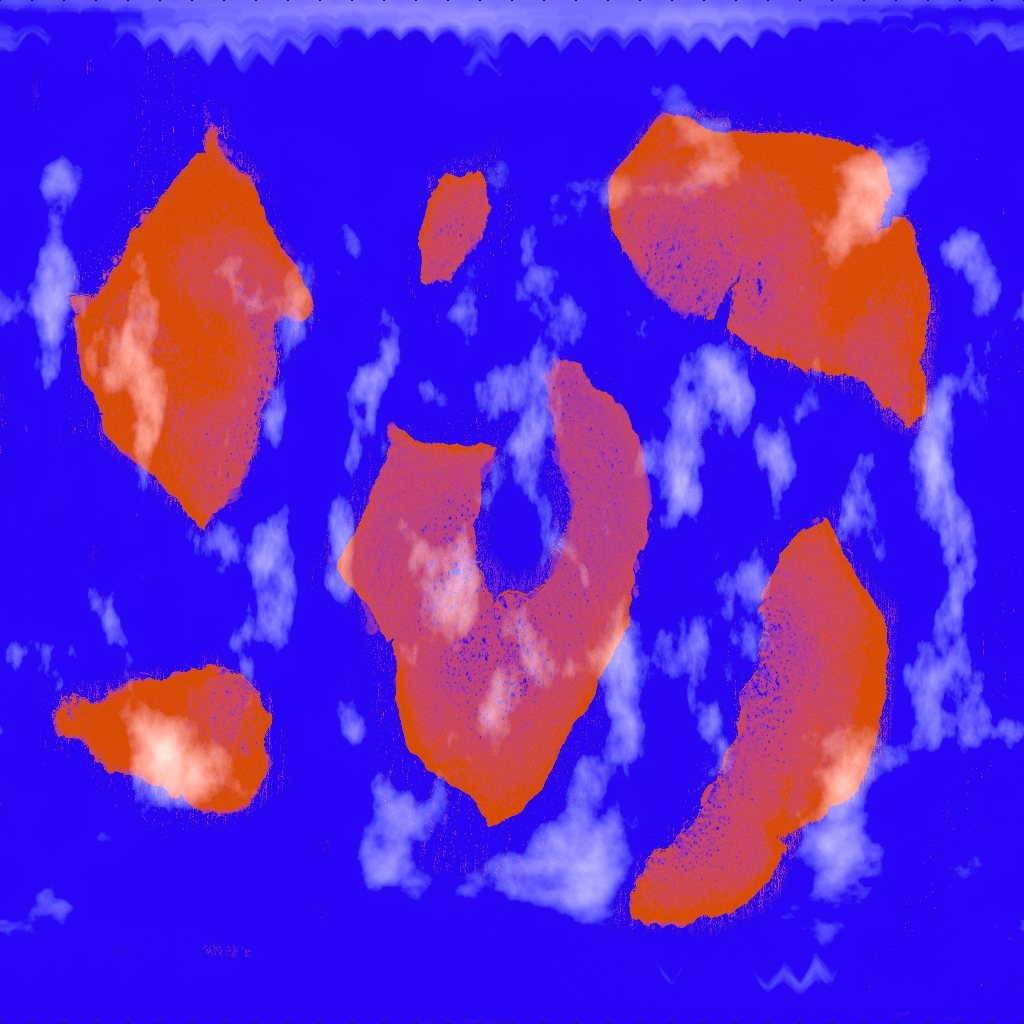
\includegraphics[width=0.7\linewidth]{Abbildungen/Weltenbau/Welt/gara-map}
	\caption[Weltkarte von Gara]{\textbf{Die Weltkarte von Gara.}}
	\label{fig:gara-map}
\end{figure}


\subsection{Serro} \label{sec:mond}
Serro ist ein Gesteinsbrocken, dessen Zusammensetzung aus Gestein und metallischen Erzen für sein charakteristisches Erscheinungsbild sorgt.



\section{Kontinent}
Der Kontinent auf dem wir sind ist Teil von der Landmasse, die sich einmal um den ganzen Planeten spannt.
Er befindet sich auf mittleren Breitengraden ziemlich mittig bezüglich des Mittelpunktes des Planetensystems.
Dadurch haben wir dort etwa mitteleuropäische Voraussetzungen was Jahreszeiten und Temperaturen anbelangt.

\subsection{Das Riesengebirge}
Ein gigantisches Gebirge, das Riesengebirge, prägt das Bild des Kontinents.

\subsection{Gigantus Wald} \label{sec:gigantuswald}
\begin{outline}
	\1 wie bekannt, können auch Pflanzen die ihnen innewohnende Magie nutzen. Eine Art (!!) von Bäumen haben folgendes entwickelt: sie ermöglichen mittels der Magie die Wasserversorgung der oberen Baumabschnitte gegen die Gravitation. Das Größeneinschränkende Element normaler Bäume ist damit weg. Daher konnten die Bäume extrem groß werden, bevor weitere Prozesse ihr Wachstum stoppten und hatten damit den Platz an der Sonne sicher
	\1  diese Garganten (Working title) erreichen Höhen von 500m und ähnlich wie aus dem Dschungel bekannt, bilden sich somit verschiedene vertikale Lebensbereiche
	\1 der Boden ist bedeckt mit allerlei Gehölz und Sträuchern, die wenig Sonnenlicht brauchen, und ganz vorne voran riesigen Pilzen, die in Symbiose mit den riesigen Bäumen ebenfalls ein gigantisches unterirdisches Netzwerk bildeten und nun gigantische Fruchtkörper (:mushroom:  das da) ausbilden können
	\1 die ersten kräftigen Äste der Garganten haben stark grüne, mit viel Chlorophyll gefüllte Blätter, die jegliches Licht, das durch die oberen Schichten kommt, aufnehmen kann. Für unsere Verhältnisse stehen die Bäume zwar ewig weit auseinander, doch auf ein normales Größenverhältnis reduziert nicht. Ihre Äste können sich an den Spitzen erreichen und bilden so mittels der Äste und den riesigen Laubblättern eine Art zweiten Boden, beginnend in 200m Höhe
	\1 durch die Ausmaße der Äste sammelt sich Erde hier und dort und es wachsen normale Bäume auf dieser Ebene, allerdings nicht zu weit vom Stamm der Garganten entfernt. Ebenso finden sich hier normale Büsche etc. Schlingpflanzen ziehen sich um die dicken Äste und es bildete sich so im Laufe der Zeit in dicker "Boden" - mit unerwartete Löchern hier und da
	\1 Da wir uns hier schon in der Krone der Bäume befinden, ist ab dieser zweiten Schicht ein langsamer Verlauf in den folgenden 300m: Die Baumkrone begünstigt in ihren Ausmaßen das Wachsen anderer Bäume, Sträucher, Kräuter etc, insbesondere parasitischer Lebensformen wie Schlingpflanzen und Misteln. Auch einige "normale Bäume" wachsen nicht nur auf den Erdansammlungen, sondern auch in das Holz der Äste hinein. Insgesamt bildet sich so wie eine Art Gerüst, welches aus festen "Platformen", aus festen und wackligen Wegen horizontal, vertikal und schräg, aus Bereichen lockerer Vegetation (wie Lianen) und aus "Lichtungen" (3D, nicht 2D) besteht.
	\1 nach oben hin werden die Blätter der Garganten immer lichtdurchlässiger. Die untersten Blätter sind mehrere Meter dick und dunkelgrün vor Chlorophyll. Die obersten sind nur ein paar Zentimeter dick, kleiner, leicht hellgrün gefärbt und ansonsten Lichtdurchlässig. Das sorgt dafür, dass das Licht bis unten hin durchkommt und effizient genutzt werden kann, um den riesigen Baum (und seine Parasiten) zu versorgen
	\1 ebenso wie die Fauna, hat sich hier auch viel Getier angesammelt und angepasst in den verschiedenen Stufen. So nisten bestimmte Vögel nur in den oberen 50m der Baumkronen. Auch ein paar Menschen fanden sich hier vor langer Zeit ein und haben sich an das Leben in den Baumkronen (von 200-350m etwa) angepasst. Es ist die Heimat der \npref{rasse:sylvan}.
	\1 allerdings ist dann doch der einschränkende faktor zum einen die stabilität von holz, bevor der baum unter der eigenlast zusammenbricht, und die biegsamkeit von holz, bevor höhenwinde den baum zerbrechen. gegen letzteres könnte der baum natürlich einfach sehr dick sein. mit werten, die ich jetzt auf die schnelle für holz gefunden hab, sollte das ganze bei wenigen hundert m höhe schon instabil werden. man könnte vielleicht argumentieren, dass der baum nicht nur wasser besser transportieren kann, sondern auch mineralstoffe, um seine stabilität zu erhöhen. dann hätte man gleich ein inhärent sehr hartes holz in der welt. bei dieser höhe ist die breite auch fast egal (solange sie wenige meter überschreitet)
\end{outline}

\section{Mantodea} \label{sec:land}

\section{Tal}
\begin{outline}
	\1 liegt weit ab hinter einem dichten Wald
	\1 wurde entdeckt, weil einem Fluss/Bach gefolgt wurde, er aus dem Tal kam
	\1 schon zu Zeiten der Monarchie besiedelt, allerdings erst gegen Ende
	\1 Karte siehe Abb. \ref{fig:tal-karte}
\end{outline}

\begin{figure}[tbh]
	\centering
	\includegraphics[angle=-90,width=0.85\linewidth]{Abbildungen/Weltenbau/Welt/tal-karte.jpg}
	\caption[Karte des Tals]{\textbf{Die Karte des Tals.}}
	\label{fig:tal-karte}
\end{figure}

\subsection{Teich 1}
\subsection{Teich 2}
\subsection{Großer Wald}
\subsection{Klippe am Eingang}

 
\include{Dateien/Magie}
\include{Dateien/Essenz}
\include{Dateien/Lebensformen}


\part{Geschichte}
\chapter{Welt}
\chapter{Kontinent}
\section{Nachbarland 1}
\subsection{Kurzbeschreibung}
\begin{outline}
	\1 Name: 
	\1 Lage:
	\1 Topographie:
	\1 ansässige Rassen:
	\1 Regierung:
	\1 Wirtschaft:
	\1 politisches Verhältnis zu unserem Land: neutral, potentiell feindlich
\end{outline}

\subsection{Geschichte}
Das einstige Königreich (NaLa) wird derzeit von einer Katastrophe in die andere gejagt.
Zuerst kam es zu Aufständen gegen die Monarchie, woraus sich ein handfester Bürgerkrieg entwickelte.
Im Verlaufe dieses Bürgerkrieges kam es zu Enteignungen und viele junge Menschen verloren ihre Eltern.
Diese Situation wird nun schamlos ausgenutzt von einer militanten Bewegung (MilBe), die sich zum Ziel gesetzt hat, aus NaLa einen egalitären Staat zu machen.
Das bedeutet zwar grundlegend, dass alle Einwohner den gleichen Zugang zu den zentralen Ressourcen haben (Nahrungsmittel, Güter, Land usw.) und auch Keiner dauerhaft Macht über Andere ausüben kann.
Der soziale Status des Einzelnen soll vor allem von seinen Fähigkeiten und seinem Willen abhängen.
Es soll politische und soziale Gleichheit herrschen.
Aber damit einher geht auch, dass individueller Besitz und Eigentum nur einen nachrangigen Stellenwert haben. (Im Grunde also das Prinzip des Kommunismus.)\\
\\
Die MilBe rekrutiert viele der elternlosen Jugendlichen, die ohne Bindungen dastehen sowie Personen, die aufgrund der Enteignungen und des Bürgerkrieges keine Verbindungen zu anderen Gemeinschaften mehr haben.
Außerdem verfolgt die MilBe eine stark nationalistische Philosophie, möchte Minderheiten im eigenen Land unterdrücken und ausmerzen und das eigene Volk von Fehlerhaftigkeit befreien.
Zu einer der zu bekämpfenden Fehler gehören alle Magiebegabten, die sich gegen die MilBe stellen, da sie über zu viel Macht verfügen.
In den eigenen Reihen hingegen sieht die MilBe sehr gerne, mächtige und regimetreue Magier.\\
\\
Der letzte Monarch wurde vor kurzem durch einen blutigen, durch die MilBe angeführten Aufstand ins Exil (unser Land oder ein anderes?) vertrieben.
Jetzt beginnt die MilBe die politische Säuberung von NaLa und verfolgt, foltert und ermordet Anhänger, Sympathisanten und Unterstellte der Monarchie und des Monarchen.
Die Hauptstadt von NaLa ist bereits eingenommen und eine „Demokratie“ ist ausgerufen worden, mit dem Anführer der MilBe als Staatsoberhaupt.\\
\\
Nach den langen Kämpfen begrüßt ein Großteil der Bevölkerung nun die Truppen der MilBe jubelnd.
Ein großer Teil der Kämpfer bestand aus Kindersoldaten, die zu diesem Zeitpunkt nichts anderes als ein Leben als Soldat kannten.
Doch diese Stimmungslage kippt sehr schnell als das Staatsoberhaupt mit seinem Terrorregime beginnt.
Die Besonderheit daran: Im Gegensatz zu anderen Diktatoren will dieser sich nicht zu erkennen geben und verbirgt sich hinter den Reihen der MilBe und einer großen Regierungsstruktur.
Damit will er vermeiden, dass Anschläge gegen ihn ausgeführt werden.\\
\\
In dieser Zeit, in der das Terrorregime beginnt, befindet sich NaLa aktuell.\\
\\
Die Hauptstadt wurde komplett „evakuiert“ und die MilBe hat sich dort niedergelassen.
Wer im Verdacht steht, mit Magiern, Minderheiten wie den Zwergen, Monarchieverfechtern oder sogar Ausländern/anderen Rassen zu kollaborieren, wird mitsamt der ganzen Familie (Ehegatten und Kinder) ermordet.
Anfangs werden sie klassisch hingerichtet, doch das Metall ermüdet schnell und die MilBe will Ressourcen sparen.
Darum werden die Menschen (soll es diese oder eine andere Rasse sein?) brutal zu Tode geprügelt.
Kinder werden einfach mit den Köpfen gegen Bäume geschlagen oder von Klippen gestoßen.
Erwachsene werden gehängt, oder je nach belieben anderweitig waffenfrei ermordet. Zuvor jedoch werden alle maßlos gefoltert, um Informationen über weitere Gegner der Regimes zu erhalten.
Gefangenenlager werden errichtet und täglich hunderte Menschen(?) getötet.\\
\\
Alle übrigen Mitglieder der Gesellschaft, die nicht zur MilBe überlaufen, werden in Arbeitslager gezwungen und der bisherige Reichtum, die Infrastruktur und alles, was sich bisher in NaLa entwickelt hatte, soll niedergerissen und neu strukturiert und aufgebaut werden.
Ganz nach den Vorstellungen der MilBe.\\
\\
Aufgrund dieser Entwicklungen ist NaLa gerade vollauf mit seinen eigenen Problemen beschäftigt und wird sich aktuell weder mit unserem Land verbünden noch sich anfeinden – zumindest vorerst!
Allerdings werden mittellose Flüchtlinge in unser Land kommen, die von dort berichten und Schreckliches erlitten haben.

\subsection{Gräueltaten}
Die MilBe-Soldaten, meist jung und vom Land, trieben die Menschen(?) ohne Gnade aus der Hauptstadt.
So auch Kranke, die teilweise noch verbunden waren und deren Binden von Blut durchtränkt, teils von Angehörigen auf ihren Bahren stadtauswärts getragen, andere wiederum versuchten auf allen Vieren zu krabbeln, weil sie keine Verwandten mehr hatten und nicht mehr gehen konnten.\\
\\
Neben den Massenmorden ist eine weitere Methode der MilBe der Tod durch Arbeit.
In den Arbeitslagern müssen die Gefangenen bis zur letzten Kraft arbeiten, wer nicht mehr kann, wird aussortiert oder zum Sterben zurückgelassen.
Viele sterben in den Lagern an Unterernährung, Seuchen, Überarbeitung und Folter.\\
\\
Wer in den Lagern ankam, wurde so lange gefoltert, bis er mindestens 50 bis 60 Personen denunziert hatte.
Diese wurden dann wiederum gefangen genommen usw.\\
\\
Zwangsehen um Verwandtschaftsverhältnisse zu schwächen und den Gehorsam gegenüber der MilBe zu stärken.
Bei der Zeremonie müssen die Eheleute sagen: „Ich danke MilBe, dass sie mir gute Eltern sind und mir erlauben, einen Partner zu haben und sich um mich kümmern, als wäre ich ihr biologisches Kind.“\\
Wenn eine Frau Angst hat oder schlichtweg keinen Sex mit ihrem neuen Ehemann haben will, darf sie gefoltert oder eingesperrt werden.
Der Mann kann sich beschweren, dass er um den Vollzug der Ehe betrogen wurde oder aber der Vorfall wird der MilBe von einem Spitzel gemeldet.
Die Folgen des Verstoßes sind nicht absehbar, weshalb es in den Augen vieler Frauen besser ist, den erzwungenen Geschlechtsverkehr, der vom Staat verlangt wird, einfach geschehen zu lassen.\\
\\
Babys von Verrätern werden nicht behalten.
Sie könnten später Rache nehmen.
Darum werden sie von Untergebenen der MilBe an den Füßen gepackt und gegen Bäume geschleudert.

\section{Nachbarland 2}
\subsection{Kurzbeschreibung}
\begin{outline}
	\1 Name: 
	\1 Lage:
	\1 Topographie:
	\1 ansässige Rassen:
	\1 Regierung:
	\1 Wirtschaft:
	\1 politisches Verhältnis zu unserem Land: freundlich
\end{outline}

\subsection{Geschichte}

\section{Nachbarland 3}
\subsection{Kurzbeschreibung}
\begin{outline}
	\1 Name: 
	\1 Lage:
	\1 Topographie:
	\1 ansässige Rassen:
	\1 Regierung:
	\1 Wirtschaft:
	\1 politisches Verhältnis zu unserem Land: freundlich
\end{outline}

\subsection{Geschichte}

\chapter{Mantodea}
\begin{outline}
	\1 Lage: 
	\1 Topographie:
	\1 ansässige Rassen: \npref{rasse:mensch}, \npref{rasse:zwerg}, \npref{rasse:sylvan}
\end{outline}
\bigskip

\begin{chronology}[startyear=-1400,stopyear=550,%
	dates=false,% Anzeigen von Start- und Enddatum der Timeline
	arrowwidth=0.01\textwidth]% Länge des Pfeilkopfes
	\setupchronoevent{textwidth=1.5cm,textstyle=\centering\small}
	\setupchronoperiode{dates=false,textstyle=\textbf,textdepth=-15pt}
	\chronograduation{300}
	\chronoperiodecoloralternation{blue,green,purple,yellow} %selbst die Farben festlegen, welche wechseln. Alternativ auch color=xy in [] hinter chronoperiode
	\chronoperiode{-1390}{-750}{Stämme}
	\chronoevent{-1300}{Menschen kommen}
	\chronoperiode{-750}{-600}{Waldvolk tot}
	\chronoevent[textwidth=2cm]{-600}{Machtergreifung Kriegsherr}
	\chronoperiode{-600}{255}{Monarchie}
	\chronoevent{-200}{Missio-nierung}
	\chronoevent{0}{Theodors Aufstieg}
	\chronoevent{255}{Machtergreifung Orden}
	\chronoperiode{485}{520}{Spiel}
\end{chronology}

\section{Stammesverbände}
Etwa 1300 vor Theodors Aufstieg wanderte ein großer Stamm aus den unwirtlichen Gefilden des Nordens weiter nach Süden.
Sie überfielen bestehende Gemeinschaften, raubten sie aus oder machten sie sich Untertan.
Die Nordlinge ließen sich umgeben von grünen Wäldern und fruchtbaren Böden entlang eines großen Flusses nieder.
Im Nordwesten wurde das von ihnen eroberte Gebiet (Mantodea) von einem riesigen Gebirgszug begrenzt und im Südosten durch einen Wald mit riesenhaften Bäumen und einer ungeahnten Ausdehnung (\npref{sec:gigantuswald}).\\
\\
Ihre Gruppe teilte sich in kleinere Stämme auf.
Einige blieben auf der Ebene am Fluss, andere zog es in die Berge, auch der dort auffindbaren Rohstoffe wegen.
Dieser lockere Verbund aus Stammesverbänden hielt lange Zeit an, auch ohne feste Struktur.
Das einzige, was sie alle miteinander verbunden hat, war die militärische Stärke.

\section{Der Untergang des dunklen Volks}
\begin{outline}
	\1 Waldvolk, Mischung aus Sylvan und Halblingen - animalisch, klein gewachsen, mit dem Wald verbunden und an ihn angepasst, leben in den Schatten tiefer, undurchdringlicher Wälder
	\1 gegen 750 vTA kommt es zu den ersten Reibereien zwischen dem ansässigen Volk und den Einwanderern
	\1 Menschen/Nordlinge bauen immer größere Siedlungen, nehmen Wald weg
	\1 Waldvolk stiehlt von Vieh und Feldern aufgrund von Nahrungsknappheit und verteidigen für sie wichtige Teile des Waldes
	\1 Unruhen verstärken sich, Eskalation
	\1 Bürgerkrieg, der gegen 600 vTA zur Auslöschung des dunklen Volkes führt
\end{outline}

\section{Monarchie}
\begin{outline}
	\1 einer der Heerführer übernimmt die Landesherrschaft
	\1 baut seine Einflüsse aus und sichert seinen Nachkömmlingen die Thronfolge --> es entsteht eine Erb-Monarchie in der viele Intrigen gesponnen, viele interne Kriege und Machtspiele geführt werden und Brudermord auf der Tagesordnung steht, um an den gewünschten Titel zu gelangen
\end{outline}

\section{Aufstieg der Religion}
\begin{outline}
	\1 um die 200 vTA erreicht ein Missionar die Gegend und beginnt, den Leuten von den 5 Göttern zu predigen
	\1 die Religion breitet sich von ihrem Startgebiet aus, bleibt aber recht beschränkt in ihren Ausmaßen
	\1 ein Teil des Adels lässt sich ebenfalls bekehren, es bildet sich eine religiöse Gemeinschaft einer Kirche
	\1 bei einem Machtvakuum durch den Tod eines Königs ohne Kinder gewinnt im Krieg einer der Adligen aus einem Haus mit ehemals königlichem Blut, welches zur Religion übertrat
	\1 dies ist das Jahr 0
	\1 es folgt eine erzwungen Missionierung des restlichen Landes: mit Waffengewalt
	\1 über die nächsten Generationen an Königen erhält die Kirche immer mehr Reichtum und Einfluss
	\1 unter den richtigen Leuten erfolgt eine strenge Strukturierung der Kirche und stärkere Auflagen im Glauben und die Macht und Mittel wachsen. Zudem gibt sie sich nun selbst einen Namen
	\1 als 253 nTA der aktuelle Monarch verstirbt und seine Kinder in einen weiteren Krieg untereinander ausbrechen, beschließt der Orden, die günstige Situation zu nutzen, mobilisiert die Ressourcen und stürzt die Königsfamilie
	\1 das Land wird nun vom obersten Priester der 5 regiert
\end{outline}

\section{Herrschaft des Ordens}
\begin{outline}
	\1 im Verlauf der ersten Jahrzehnte organisiert sich der Orden neu und bildet nach und nach die heutigen Strukturen heraus: die Regierung von einem Priester mit 4 weiteren
	\1 es bildet sich eine kommunistische Grundstruktur für die Führung der Bevölkerung aus. Dabei wird keiner hängen gelassen, solange er seine Arbeit gewissenhaft erledigt
	\1 weitere Anordnungen des Ordens (Bluttausch über junge Leute, Anordnungen zur Landwirtschaft, etc) führen zu einer insgesamt verbesserten Lebenssituation mit deutlich weniger Hungerperioden
	\1 die militaristische Führung spaltet sich ein wenig von der Geistlichen ab, wobei sie dieser noch untergeordnet ist
	\1 Aufbau von Ausbildungsstätten für magiebegabte junge Menschen
	\1 Aufbau einer Heeresstruktur mit Ausbildung junger Rekruten
\end{outline}

\section{Aktuell}
\begin{outline}
	\1 innerhalb des Ordens außerdem Machtkampf der Magie-Häuser
	\1 Orden wirbt auch in Nachbarländern an, hauptsächlich aus bildungsferner und mittelloser Schicht.\\
	Eltern sind leichter mit Naturalien und monetären Mitteln auszuzahlen als reiche, gebildete Familien mit geringerer Kinderzahl
	\1 Rebellion gegen Gottglauben und den Klerus bildet sich
	\1 Das dunkle Volk existiert nur noch als Ammenmärchen.
\end{outline}

\section{Nahe Zukunft}

\section{Ferne Zukunft}

\chapter{Tal}

\part{Gesellschaft}
\chapter{Religion}
\section{Übersicht}
\begin{outline}
	\1 Der Glaube an 5 gute und 2 böse Götter.
	\1 Das Symbol der Religion ergibt sich wie in Abschnitt \npref{sec:goettersymbol} erklärt aus dem Zusammenspiel der 7 Götter und ist in Bild \ref{fig:goettersymbol} dargestellt.
\end{outline}

\section{Geschichte}
Die hier erzählte Geschichte ist die vom Klerus verbreitete Sage über die Entstehung der Götter des Streits und der Heimtücke. \\\\
Es ist unklar, wie die Götter entstanden sind. 
Es geschah irgendwie irgendwann. 
Auf der noch recht unbewohnbaren Erde formten sie lebensfreundliches Gebiet mit ihrer jeweiligen Magie. 
Sie erschufen das Leben und ließen ihm seinen eigenen Lauf.\\
Nachdem sie jedoch viel Zeit damit verbracht hatten, sich an ihrem Paradies zu ergötzen, wollten sie auch Wesen nach ihrem Abbild schaffen und so lenkten sie das Leben und die Natur und brachten dadurch die Menschen hervor. 
Die Menschen, intelligent genug um Kultur aufzubringen, verfielen jedoch in viele Kriege. 
Mitgerissen aufgrund ihrer Ähnlichkeit und weil sie die Menschen so interessant fanden, integrierten sich die Götter in diese Streitigkeiten. 
Dabei nahmen sie die Positionen ihrer Menschengruppen an und halfen ihnen und wurden so langsam auch in einen Streit untereinander gezogen, wobei sie ihre negativen Seiten ausspielten.\\
Dies äußerte sich in vielen kleinen Dingen \textbf{(hier Geschichtchen einfügen)}, bis die Götter schließlich merkten, dass es so nicht weiter gehen kann. 
Sie setzten sich zusammen und kamen zum Schluss, dass sie, um wahre Leiter und Lenker des Lebens zu sein, ihre negativen Aspekte los werden müssten. 
Andernfalls würden ihre dunklen Seiten sie immer wieder übermannen können, was bereits große negative Folgen für alle Lebewesen hatte und auch wieder haben könnte.\\
Darum bereiteten die Götter ein Ritual vor, um perfekt zu werden und sich wortwörtlich von ihren schwachen Seiten rein zu waschen. 
Dazu begaben sie sich in einen See weitab der Zivilisation. 
Sie wuschen ihre schlechten Seiten von sich ab und versiegelten diese im See. 
\textbf{Allerdings gab es ein kleines Leck, durch welches kontinuierlich ein wenig von der Magie und dem Schlechten austrat.}\\
Danach treten die Götter lange Zeit nicht in Erscheinung. 
In der Nähe des Sees, den Bach hinunter, lebte ein Paar. 
All sein Trinkwasser nahm es aus dem Bach und all ihre Ernte wurde mit dem Wasser bewässert. 
So nahmen sie über Zeit immer mehr von dem Bösen in sich auf.
So wie ihre Macht und Magie wuchs, tat es auch das Böse in ihnen und verzehrte ihre guten Geister. 
Sie begannen aktiv das Böse aus der Umwelt und schließlich dem See zu absorbieren und wurden immer mächtiger und verdorbener. 
Sie führten Verwüstung und Zwist herbei und die Götter wurden auf sie aufmerksam. 
Ihre Versuche, sie zu bekämpfen und unter Kontrolle zu bekommen, scheiterten unter großen Verlusten in der Umwelt. 
Schließlich sahen die Götter ein, dass sie die beiden nicht besiegen konnten und unter all ihrer gebündelten Macht, um alle Lebewesen zu schütze, ersannen sie einen radikalen Plan.\\
Da die Götter zu verantworten hatten, dass diese Monster auf die Welt kamen, sahen sie es als ihre Pflicht, die Welt auch wieder von ihnen zu befreien. 
Aufgrund der zuvor genannten Umstände war die Maßnahme jedoch von drastischer Natur: sie hoben den Ort, auf dem sie die beiden bekämpften, aus der Erde heraus in den Himmel. 
Dort werden sie nun für alle Zeit gegen die beiden kämpfen und sie in Schach halten, damit das Leben auf der Erde geschützt ist.\\
Doch die beiden Bösen versuchen ihre Macht zu vergrößern, indem sie ihre Aktuelle auch dazu nutzen, den Lebewesen auf der Erde Böses einzuflüstern und sie zu manipulieren. 
\textbf{Die Erdenwesen sollen ihnen dienen.}\\
Bevor die guten Götter die Erdmasse mitsamt den Bösen in den Himmel aufgehoben haben, \textbf{erschufen sie gemeinsam einen Führer für die Toten}, der die verstorbenen Seelen zu ihnen bringen soll. 
Im Laufe der Zeit, in der sie ihre Pflichten als Götter und Führer der Welt etwas außen vor ließen, haben sie es geschafft, die Bösen zurück zu treiben. 
Nun gibt es nur noch Kampf auf einem kleinen Teil des Himmels-Brockens.\\
Nachdem die Toten verbrannt wurden, steigen ihre Seelen in den Himmel auf.
Wenn die Verstorbenen in ihrem Leben gut waren und sich nicht von den Einflüsterungen der bösen Götter haben verführen lassen, werden sie vom Seelenleiter hinüber geführt, auf dass sie mit ihrer Kraft die Götter unterstützen und in ihrem Paradies wohnen können. 
Die verdorbenen Seelen jedoch werden vom Seelenleiter zu Serro fehlgeleitet, damit sie nicht den Bösen helfen können, und auf dem Mond festhängen müssen.

\section{Götter}
In dem Land, in dem wir uns befinden, gibt es mehrere Götter. 
Regional unterscheidet sich die Wahl der bevorzugten Götter.
Diese sind Fiktion und existieren nicht wirklich; es gibt also auch keine Wunder, die von ihnen gewirkt werden. 
Allerdings interpretieren Menschen ja gerne sehr viel und sehen deshalb ein paar Dinge als Wunder an, die z.B. von den Priestern gemacht werden. 
Weil diese Priester gute Magier sind, aber das alles natürlich als Geschenk der Götter sehen.\\

Die Ausführungen im Folgenden stellen den Pantheon dar, wie er zur Zeit des Spiels angebetet wird.
Alle Namen sind vorläufig und mehr Möglichkeit gesehen, den Göttern und benannten Orten etwas mehr Griffigkeit zu geben.
Die Details, die im Folgenden gegeben werden (insbesondere die beispielhafte Mythen und Erzählungen über die Götter) dienen der Anschaulichkeit für uns und müssen sich nicht zwingend im Spiel wiederfinden.




\subsection{Asdir -- Gott der Führung und des Schutzes}
Asdir ist der Anführer der Götter - nicht aufgrund außergewöhnlicher Stärke oder Charisma - Asdir ist nicht mächtiger als seine Mitgötter, sondern weil es seinem Wesen entspricht. 
Asdir ist standhaft, mutig und vertritt Führung durch Vorbild. 
Da, wo die Schutzbedürftigen verteidigt oder Verlorenen angeleitet werden müssen, ist Asdir in der ersten Reihe zu finden.
\begin{outline}
	\1 Aussehen (Abb. \ref{fig:asdir})
		\2 großer Mann im mittleren Alter
		\2 kurze silberne Haare
		\2 häufig in Rüstung und mit alten Kampfnarben
	\1 Aspekte
		\2 Herrschaft und Führung
		\2 Kampf und Schutz
		\2 Vertreibung von Übel
	\1 Tugenden Asdirs
		\2 Standhaftigkeit, Mut
		\2 körperliche Stärke und Macht
		\2 Opferbereitschaft
	\1 Symbole
		\2 Farbe Blau
		\2 Edelstein Saphir
	\1 positive Gemüter: Mut, Macht, Kraft, Würde, Standhaftigkeit, Entscheidungsvermögen, Führungsqualitäten, Sicherheit, Intuition, Schutz
\end{outline}

\subsubsection{Weit bekannter Mythos Asdirs}
Vor Urzeiten, als die Welt noch jünger war, streiften mächtige Monster durch die Lande und verbreiteten Angst und Schrecken. 
Es begab sich, dass Asdir, als einfacher Wanderer verkleidet, in einem Dorf Herberge suchte. 
Ein Lindwurm, eine mächtige Bestie mit einer geschuppten Haut härter als Stein und Klauen und Zähnen größer und schärfer als das beste Schwert der Menschen, fiel über das Dorf her, getrieben von unstillbarer Gier und Hunger. 
Und Asdir offenbarte sich in seiner Rüstung und sprach: 
``Wer bereit ist, sein Heim und seine Familie zu verteidigen, der nehme seine Waffe und kämpfe an meiner Seite.'' 
Und die Menschen folgten seinem Ruf, gewappnet mit jedweder Waffe die sie finden konnten. 
Der Kampf war lang und schwierig und manch einer wäre dem Hunger des Wurms zum Opfer gefallen, wenn Asdir die Angriffe nicht mit Schild und Rüstung abgefangen hätte. 
Doch mit seinem letzten Atemhauch gelang es dem Lindwurm noch, Klaue an Asdir zu legen und ihm eine weitere Narbe zu verpassen.





\subsection{Rhena -- Göttin des Ausgleichs und der Gerechtigkeit}
Rhena lehrt die Menschen, die Bindungen zu ihren Mitmenschen ausgewogen zu halten. 
Sowohl Respektlosigkeit als auch übermäßige Ehrerbietung versäuern das Verhältnis zu den Mitmenschen und müssen daher vermieden werden. 
Dazu gehört, sich an die Gesetze und Regeln der Gesellschaft zu halten.
\begin{outline}
	\1 Aussehen (Abb. \ref{fig:rhena})
		\2 alte Frau  -> "weise Frau"
		\2 hochgewachsen und hager
		\2 Gehstab/ Stecken
	\1 Aspekte
		\2 Gesetzgebung und Rechtsprechung
		\2 Handel
		\2 Weises Vorgehen \footnote{Leichte Überschneidung mit Faelans Aspekt}
	\1 Tugenden Rhenas
		\2 Disziplin und Respekt
		\2 stoisch und gelassen
		\2 streng mit sich selbst und Anderen
		\2 reich an Erfahrung
	\1 Symbole
		\2 Farbe Lila
		\2 Edelstein Amethyst
	\1 positive Gemüter: Höflichkeit, Disziplin, Gleichgewicht, Ruhe, Gelassenheit, Geduld, Wachstum, Ausgeglichenheit, Strenge, Heilung, Ausgleich, Urteilvermögen
\end{outline}

\subsubsection{Weit bekannter Mythos Rhenas}:
<Rhena fällt eine Richtspruch über ...>


\begin{figure}[tbh]
	\begin{minipage}[][][b]{0.49\textwidth}
		\centering
		\vspace{0pt}
		\vspace{\baselineskip}
		\vspace{\baselineskip}
		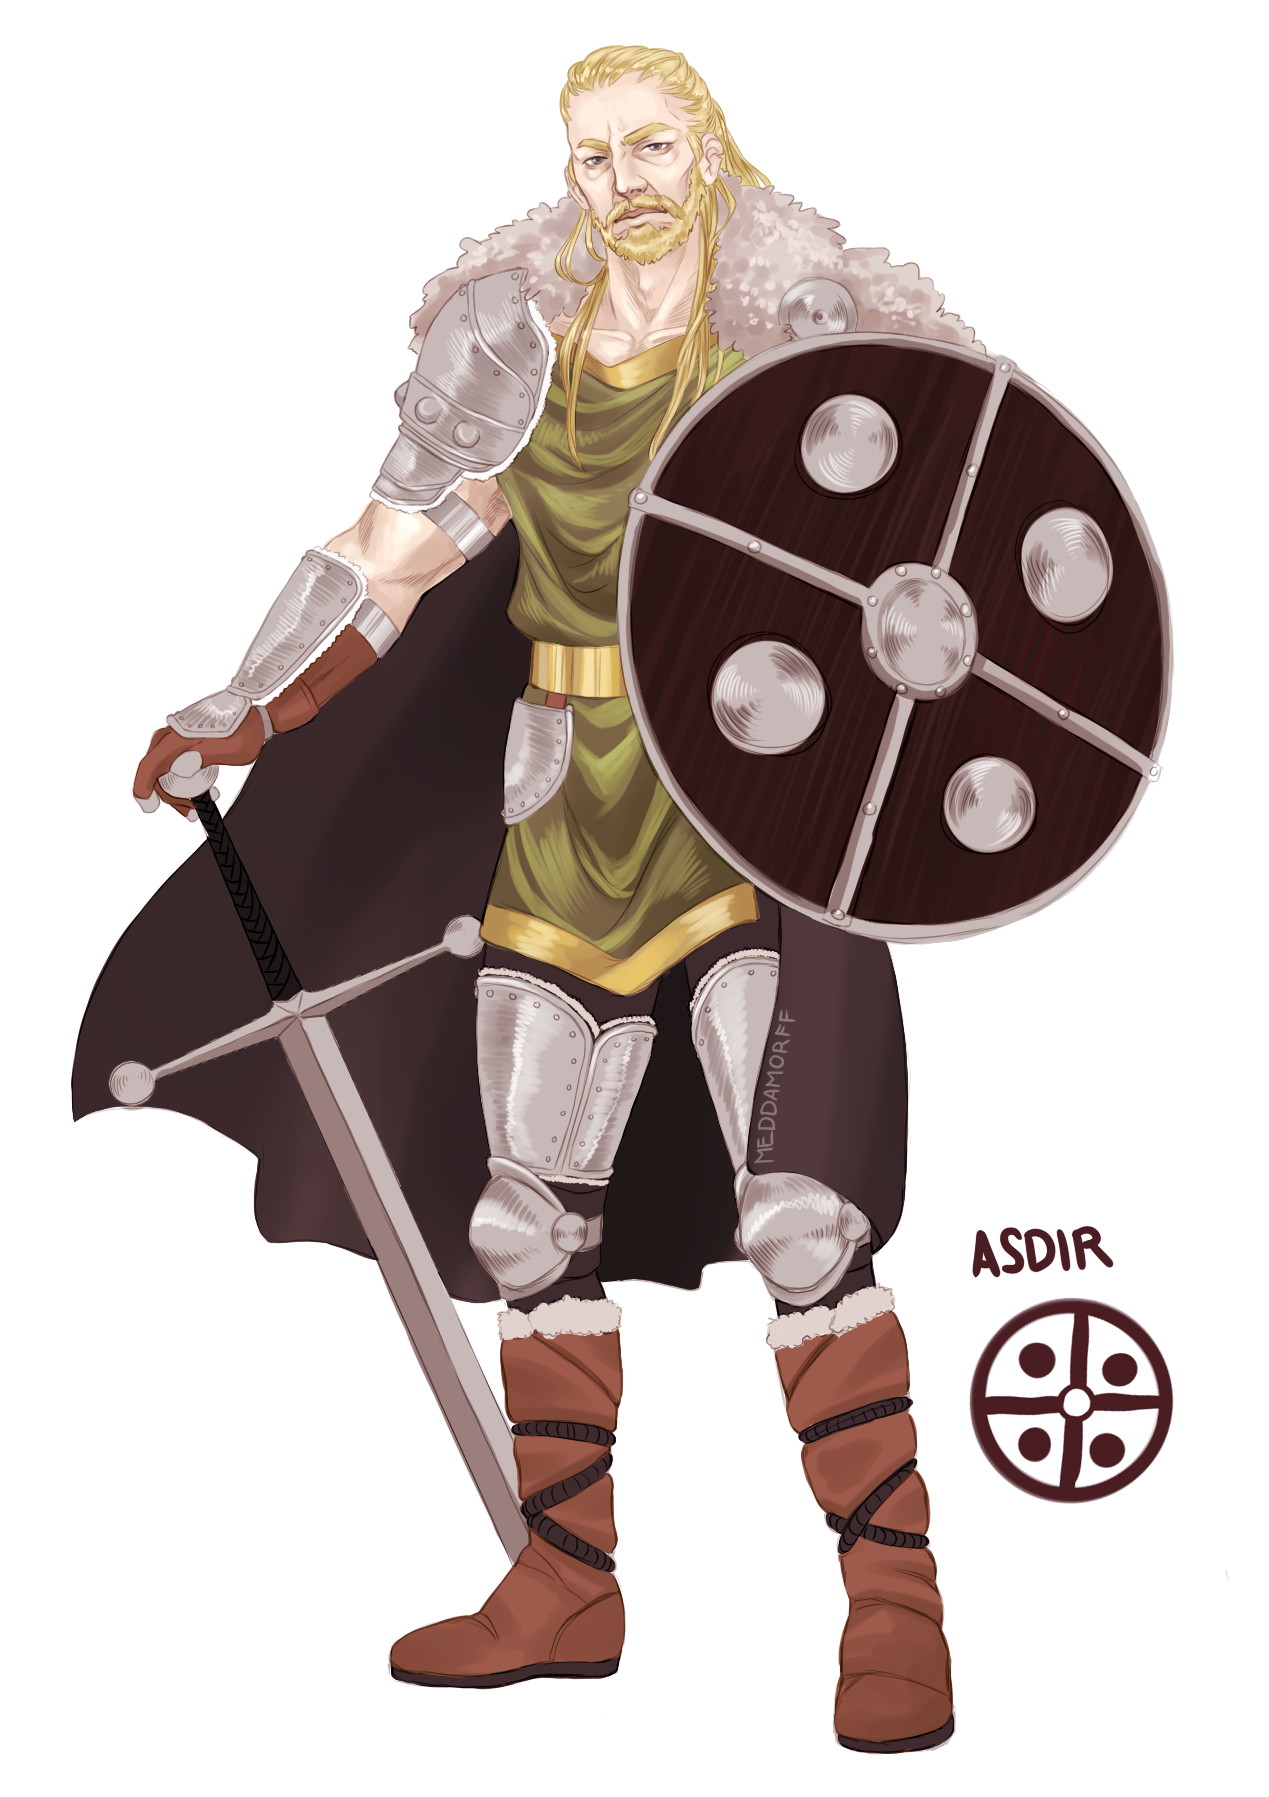
\includegraphics[width=0.94\linewidth]{Abbildungen/Gesellschaft/Religion/asdir}
		\captionsetup{width=0.95\linewidth}
		\caption[Asdir -- Gott der Führung und des Schutzes]{\textbf{Asdir -- Gott der Führung und des Schutzes}}
		\label{fig:asdir}
	\end{minipage}
	\hfill
	\begin{minipage}{0.49\textwidth}
		\centering
		\vspace{0pt}
		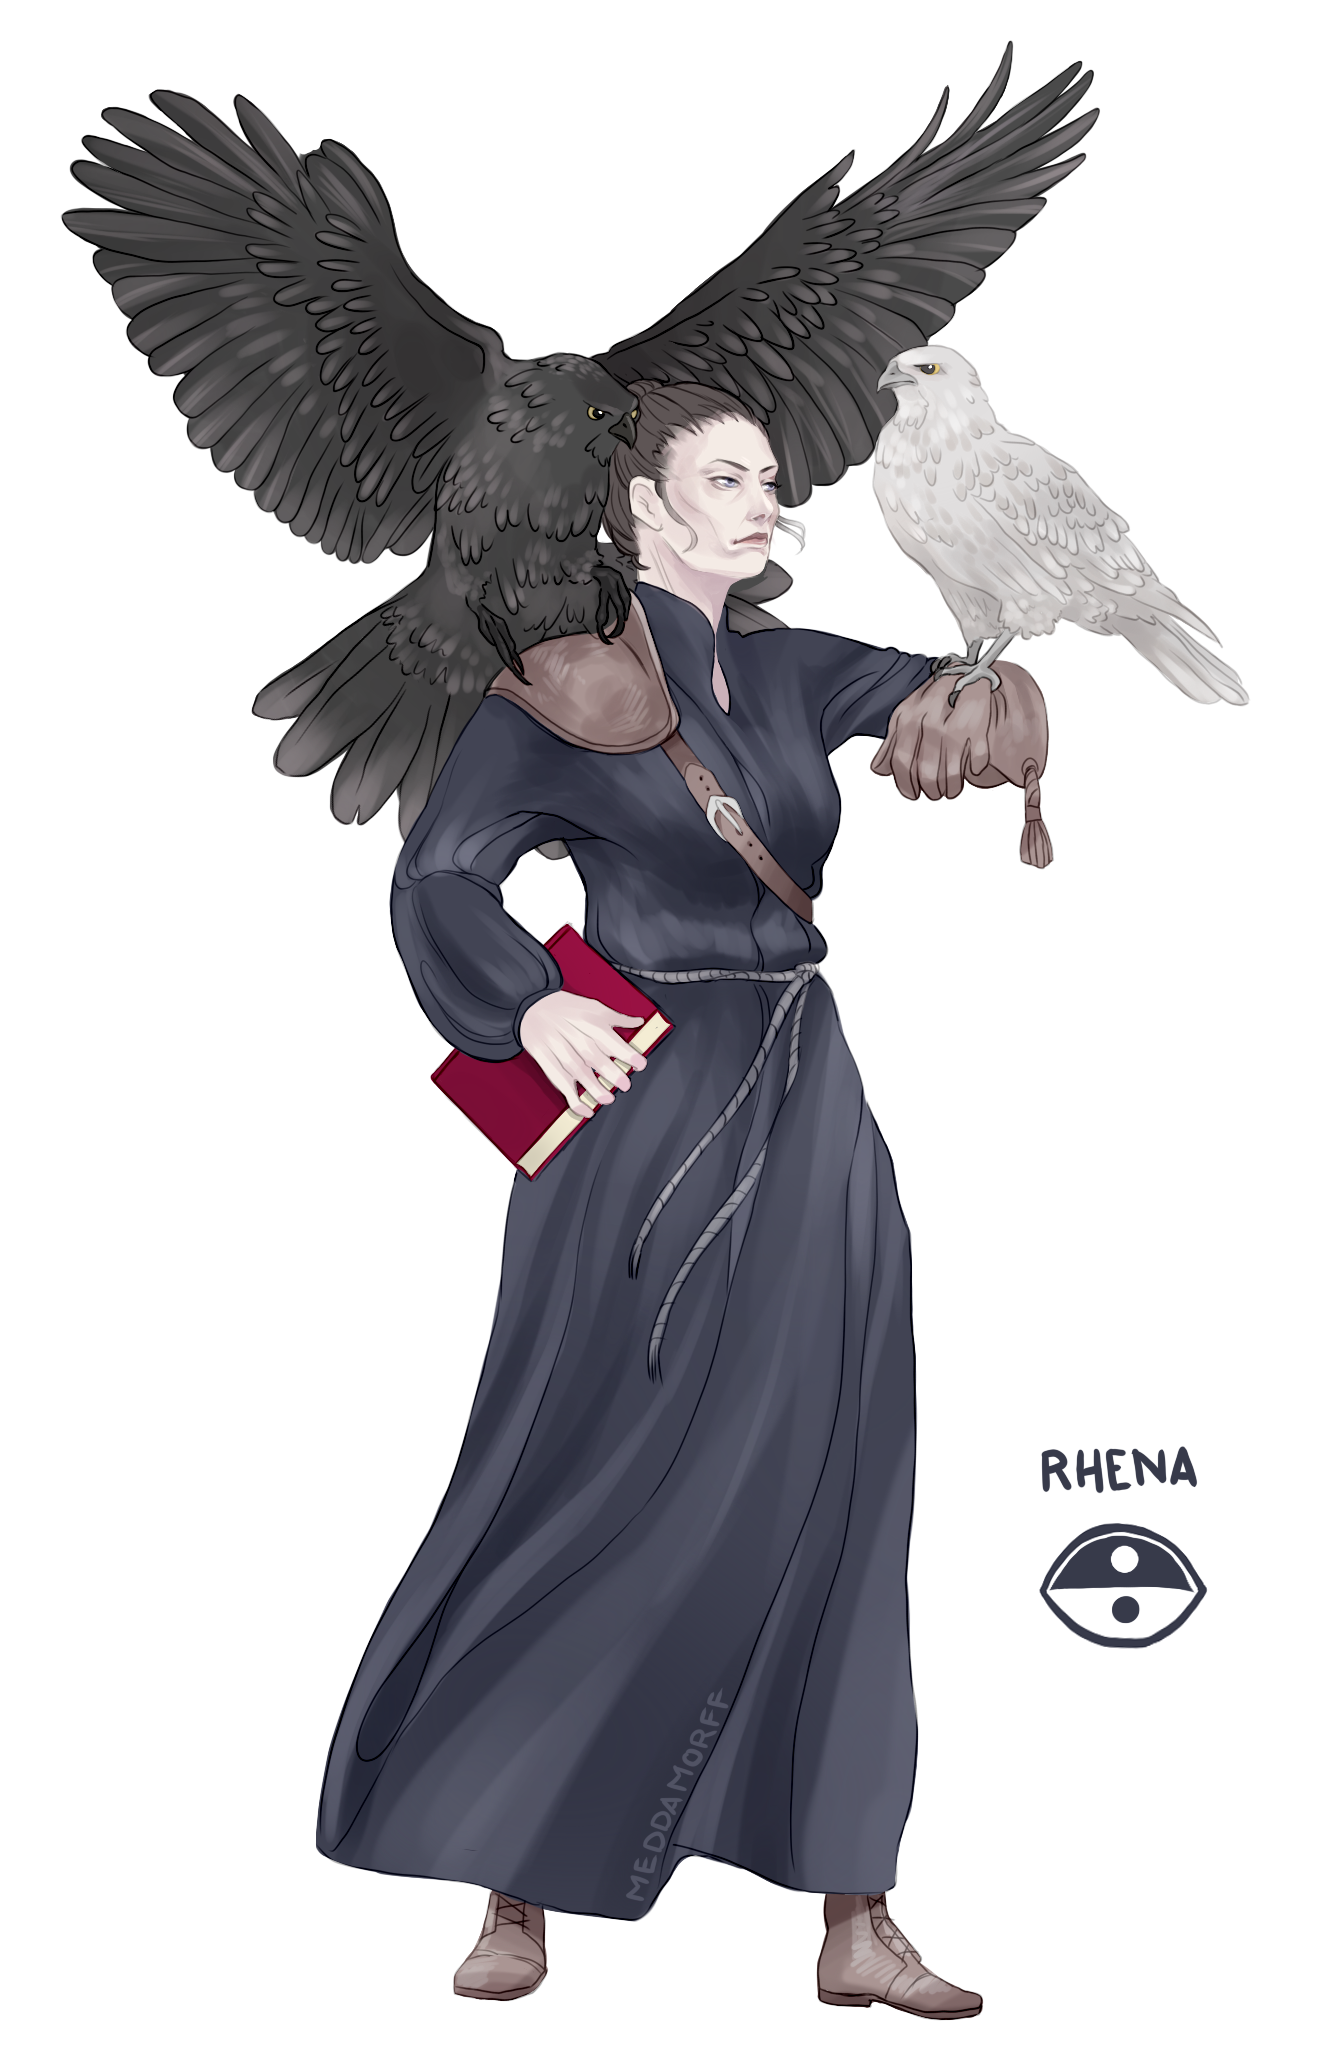
\includegraphics[width=0.94\linewidth]{Abbildungen/Gesellschaft/Religion/rhena}
		\captionsetup{width=0.95\linewidth}
		\caption[Rhena -- Göttin des Ausgleichs und der Gerechtigkeit]{\textbf{Rhena -- Göttin des Ausgleichs und der Gerechtigkeit}}
		\label{fig:rhena}
	\end{minipage}
\end{figure}


\subsection{Bouda -- Göttin der Harmonie und des Wachstums}
Bouda [gesprochen: Bo-uda] ist die schaffende Gottheit des Pantheons. 
Nach ihrem Willen erwachsen neue Pflanzen in jedem Frühling, um den Hunger aller zu stillen. 
Nach ihrem Willen wird das Band der Ehe geformt, das zwei Menschen in Harmonie miteinander verbindet. 
Bouda akzeptiert alle als ihre Kinder und schenkt die Fähigkeit, zu vergeben und zu versöhnen.
\begin{outline}
	\1 Aussehen (Abb. \ref{fig:bouda})
		\2 ``Mutterfigur''
		\2 mittleres Alter 
		\2 kräftige Figur
		\2 alltägliche Kleidung 
	\1 Aspekte
		\2 Familie (Ehe und Elternschaft)
		\2 Ernte und Wachstum
		\2 Heilung
	\1 Tugenden Boudas
		\2 Gnade und Demut
		\2 Offenheit und Akzeptanz
		\2 nichterotische Liebe
	\1 Symbole
		\2 Farbe Grün
		\2 Edelstein Smaragd
	\1 positive Gemüter: Familie, Liebe, Selbstlosigkeit, Gnade, Mitgefühl, Vergebung, Demut, Reinheit, Frieden, Toleranz, Geborgenheit, Harmonie
\end{outline}

\subsubsection{Weit bekannter Mythos Boudas}
Vor Urzeiten, als die Welt noch jünger war, lagen die Reiche der Menschen beständig im Streit miteinander. 
Pakte wurden geschmiedet und gebrochen, ein Herrscher folgte auf den nächsten und keiner vermochte es, andauernden Frieden zu finden. 
Doch manchmal schmiedete das Schicksal seltsame Bande: 
es begab sich nämlich, dass die Thronfolger zweier verfeindeter Reiche in demselben Wald jagten und von einem Sturm von ihren jeweiligen Wegen abgebracht und in der Hütte einer alten Frau zusammengebracht wurden. 
Und als die beiden sich der Anziehung bewusst wurden, die zwischen ihnen zu erblühen begann, baten sie die alte Frau, ihre Vermählung vor Bouda zu bezeugen, auf dass selbst ihre Väter sie nicht mehr trennen könnten. 
Und die alte Frau schenkte ihnen zur Mitgift zwei Armreife, die das Band ihrer Vereinigung darstellen sollten. 
Und als die beiden Thronfolger heimkehrten, kam Friedfertigkeit über jeden, der die Reife der beiden sah. 
Und zum ersten Mal seit langem herrschte Frieden zwischen den Nationen.

\begin{figure}[tbh]
	\begin{minipage}{0.44\textwidth}
		\centering
		\includegraphics[width=0.94\linewidth]{Abbildungen/Gesellschaft/Religion/bouda}
		\captionsetup{width=0.95\linewidth}
		\caption[Bouda -- Göttin der Harmonie und des Wachstums]{\textbf{Bouda -- Göttin der Harmonie und des Wachstums}}
		\label{fig:bouda}
	\end{minipage}
	\hfill
	\begin{minipage}{0.54\textwidth}
		\centering
		\includegraphics[width=0.95\linewidth]{Abbildungen/Gesellschaft/Religion/erlin}
		\captionsetup{width=0.95\linewidth}
		\caption[Erlin -- Gott der Lebensfreude und Liebe]{\textbf{Erlin -- Gott der Lebensfreude und Liebe}}
		\label{fig:erlin}
	\end{minipage}
\end{figure}



\subsection{Erlin -- Gott der Lebensfreude und Liebe}
Erlin mag für manche wie der schwächste der Götter aussehen - seine Mythen berichten fast ausschließlich von Festen und Kunstwerken. 
Und dennoch ist Erlin einer der beliebtesten Götter im einfachen Volk. 
Jeder Reigen zum Mittsommerfest, jedes alkoholschwangere Fest und jeder stille (und jeder weniger stille) Moment der Zweisamkeit genießt Erlins Segen und Unterstützung.

Doch neben diesen ausgelassenen Momenten schenkt Erlin auch denen Lebensfreude und Hoffnung, die diese am dringensten benötigen. 
Diejenigen, die von Trauer oder Hoffnungslosigkeit niedergedrückt werden, hilft der Glaube an das Lebenswerte, um sich wieder aufzuraffen.
\begin{outline}
	\1 Aussehen (Abb. \ref{fig:erlin})
		\2 junger Mann in Festtagskleidung
		\2 häufig zum Lachen aufgelegt
		\2 attraktiv 
	\1 Aspekte
		\2 erotische Liebe (als Vereinigung)
		\2 Feierlichkeiten
		\2 Kunst und Kultur
		\2 Trost und Hoffnung
	\1 Tugenden Erlins
		\2 Kreativität und Freigeistigkeit
		\2 zu Scherzen aufgelegt
		\2 charmant und fröhlich
	\1 Symbole
		\2 Farbe Gelb
		\2 Edelstein Bernstein
	\1 positive Gemüter: Glück, Hingabe, Enthusiasmus, Fröhlichkeit, Freiheit, Menschlichkeit, Kunst, Kultur, Charme, Kreativität, Freude
\end{outline}

\subsubsection{Weit bekannter Mythos Erlins}
Vor Urzeiten, als die Welt noch jünger war, waren die Menschen eitel aufgrund ihrer eigenen Fertigkeiten. 
Glemric, Barde und Meister seiner Zunft, war einer dieser Menschen. 
Er rühmte sich seiner Künste mit Flöte und Harfe und behauptete, dass selbst Erlin selbst nicht mit ihm mithalten könne.
Und so kam es, dass eines Abends, als die Nächte kurz und der Mittsommer nahe war, eine junger Mann vor seiner Tür stand und ihn zu einem Wettbewerb herausforderte. 
Gäste wurden geladen, um die Kunstfertigkeit der Kontrahenten zu bewerten und sich ihrer Kunst zu erfreuen. 
Doch jedes Stück, das Glemric aufspielte, vermochte sein Gast zu überbieten, bis letzlich sogar Glemric selbst einsehen musste, dass er geschlagen war. 
Noch an diesem Abend gelobte er, seine Ehre wiederherzustellen und sich bei seinem Gast zu revanchieren. 
Und so geschah es, dass Glemric ein Jahr später in derselben Nacht Erlin zu einer Revanche herausforderte. 
Und die Geschichten erzählen, dass ihre Wettstreite sich bis heute in derselben Nacht fortsetzen.





\subsection{Faelan -- Gott der Weisheit}
Weisheit kann viele Dinge bedeuten. 
Die Fähigkeit, Zusammenhänge zu begreifen und auszunutzen. 
Die Fähigkeit, den für sich selbst und Andere besten Weg zu erkennen. 
Und die Fähigkeit, aus dem Wenigen, was man hat, das Beste zu machen. 
Faelan verkörpert alle diese Aspekte. 
Einerseits ist er der Gott von Wissen und Gelehrsamkeit, der die Menschen Schrift, Wissen und Magie lehrt. 
Andererseits ist - beziehungsweise war - Faelan ein Gott der Schläue und der günstigen Gelegenheiten, der den Menschen überlegtes und zielstrebiges Handeln beibringt. 
Diese zweite Seite von Faelans Wesen ist mit dem Erstarken des Klerus immer mehr in Vergessenheit geraten, da die Verehrung eines Gottes der Diebe und Reisenden wenig erwünscht war.
\begin{outline}
	\1 Aussehen (Abb. \ref{fig:faelan})
		\2 Junger Mann 
		\2 schlank und gelenkig
		\2 beständig neugierig
		\2 Wissen: trägt ein Buch und einen Kohlestift mit sich
		\2 Schläue: Tarnkappe oder ähnliches ``Werkzeug''
	\1 Aspekte
		\2 Weisheit und Verständnis
		\2 Schrift
		\2 Philosophie und andere Wissenschaften
		\2 Magie
	\1 Tugenden Faelans
		\2 Neugierig und wissbegierig
		\2 Lehrend
		\2 weise und beobachtend
	\1 Symbole
		\2 Farbe Braun
		\2 Edelstein Tigerauge
	\1 positive Gemüter: Erleuchtung, Wissen, Verständnis, Konzentration, Wahrheit, Klarheit, (Um-)wandlung, Zielstrebigkeit, Weisheit, Aufstieg
\end{outline}
\subsubsection{Weit bekannter Mythos Faelans}
<Faelan stiehlt/vergibt einen Namen> 

\begin{figure}[tbh]
	\centering
	\includegraphics[height=0.45\textheight]{Abbildungen/Gesellschaft/Religion/faelan}
	\caption[Faelan -- Gott der Weisheit]{\textbf{Faelan -- Gott der Weisheit}}
	\label{fig:faelan}
\end{figure}




\subsection{Der Flüsternde Schatten -- Gott der Heimtücke}
Der Flüsternde Schatten -auch als ``Flüsterer'' bekannt - ist ein Gott, der aus einem Mangel an Emotionen entstanden ist.
Er ist manipulierend, rational und kühl. 
Mit einem wohlgesetzten Wispern schleicht er sich in die Köpfe der Menschen und lässt auch sie die Welt mit seinen Augen sehen. 
Und wer sich seines Flüsterns lange öffnet, der verliert Schritt für Schritt ebenso alle Fähigkeit zu eigenen Emotionen, bis der Mensch nicht viel mehr ist als ein lebender Schatten.
\begin{outline}
	\1 Aussehen (Abb. \ref{fig:fluesterer})
	\1 Aspekte
		\2 Feigheit
		\2 Gefühllosigkeit
		\2 Heimtücke
		\2 Rückgradlosigkeit
		\2 Eitelkeit
	\1 Plage
		\2 Depression und Trauer
		\2 grausames Kalkül
		\2 selbstsüchtige Hinterlist
		\2 Fanatismus
	\1 Symbole
		\2 Farbe Schwarz
		\2 Edelstein Obsidian
	\1 negative Gemüter: eingebildet, versteift, zwingend, ängstlich, heimtückisch, fanatisch, manipulativ, selbstüberschätzend, rücksichtslos, stolz, unterdrückend, hochnäsig,
	überheblich, arrogant, egoistisch, rückgratslos, feige, scheu, abhängig, Faul, gefühllos, eitel, misstrauisch, zynisch, nervös, voreilig, schadenfreudig
\end{outline}




\subsection{Drayl -- Göttin des Streits}
Drayl ist eine Göttin, die aus einem Übermaß an Emotionen erwachsen ist. 
Jedes Übermaß an Emotionen führt Menschen zu Konflikten, bei denen nicht die gute Sache im Vordergrund steht, sondern die Menschen von Drayls Willen bessessen sind.
Drayl kann in vielerlei Formen erscheinen - sei es eine Axt, die einem Krieger ultimative Macht im Blutrausch verspricht, ein Schatz, der einen Händler zu gierigem Tun verleitet oder ein schönes Wesen, das zu hemmungsloser und aggressiver Wolllust verführt.

\begin{outline}
	\1 Aussehen (Abb. \ref{fig:drayl})
	\1 Aspekte
		\2 Wut
		\2 Neid
		\2 Gier
		\2 Chaos
	\1 Plage
		\2 Mania
		\2 Jähzorn
		\2 Instabilität
	\1 Symbole
		\2 Farbe Rot
		\2 Edelstein Granat
	\1 negative Gemüter: gierig,  habsüchtig,  streitsüchtig, störrisch, grausam, aggressiv, undiszipliniert, neidisch, unberechenbar, unaufmerksam, jähzornig, wollüstig, völlernd, 
	chaotisch, instabil, manisch
\end{outline}



\begin{figure}[tbh]
	\begin{minipage}{0.51\textwidth}
		\centering
		\vspace{8pt}
		\vspace{\baselineskip}
		\vspace{\baselineskip}
		\includegraphics[width=0.95\linewidth]{Abbildungen/Gesellschaft/Religion/fluesterer}
		\vspace{\baselineskip}
		\vspace{\baselineskip}
		\captionsetup{width=0.95\linewidth}
		\caption[Der Flüsternde Schatten -- Gott der Heimtücke]{\textbf{Der Flüsternde Schatten -- der Gott der Heimtücke}}
		\label{fig:fluesterer}
	\end{minipage}
	\hfill
	\begin{minipage}{0.48\textwidth}
		\centering
		\includegraphics[width=0.95\linewidth]{Abbildungen/Gesellschaft/Religion/drayl}
		\captionsetup{width=0.95\linewidth}
		\caption[Drayl -- Göttin des Streits]{\textbf{Drayl -- die Göttin des Streits}}
		\label{fig:drayl}
	\end{minipage}
\end{figure}



\newpage
\subsection{Das Göttersymbol} \label{sec:goettersymbol}
Beim Wasser-/Reinigungsritual, dem Abtrennungsritual oder einem anderen war die Aufstellung der fünf Götter und ihr Energiefluss wie dargestellt in Abb. \ref{fig:goettersymbol}. 
Denn die stärksten und direktesten Verbindundungen/Folgen ihrer Aspekte sind so. 
Das ergibt eine liegende acht, also das Symbol für Unendlichkeit --> 8 als heilige Zahl; 
Götter und ihre Macht sind unendlich.\\
\\
Mit den zwei Bösen Göttern: diese versuchen, alles zu spalten und zu zerstören. 
Das wird deutlich durch die Linie, welche die 8 versucht zu zerschneiden. 
Zudem zeigt es aber auch, wie durch die bösen Götter und zum Schutz des Lebens, ein Stück von der Erde abgetrennt werden musste. 
Des Weiteren mahnt es, wie unsere Schlechten Seiten immer Versuchung und Untergang sind — aber sie sind auch ein Teil von uns und wir müssen lernen, damit umzugehen und ihnen zu widerstehen. 
Aus diesen Aspekten ergibt sich das endgültige Göttersymbol wie dargestellt in Abb. \ref{fig:goettersymbol}.\\

\begin{figure}[tbh]
	\centering
	\includegraphics[width=0.7\textwidth]{Abbildungen/Gesellschaft/Religion/goettersymbol}
	\caption[Das Symbol der Götter]{\textbf{Gestaltung und Herkunft des Symbols der Religion}\\
	Links ist die Aufstellung der Götter während des Reinigungsrituals dargestellt. H = Harmonie alias Bouda, A = Ausgleich alias Rhena, S = Schutz alias Asdir, F = Freude alias Erlin, W = Weisheit alias Faelan.\\
	Rechts ist die einfachste Form des Religionssymbols. Hier sind die zwei bösen Götter hinzugekommen, dargestellt durch den senkrechten Strich, welcher die Acht der guten Götter teilen will.}
	\label{fig:goettersymbol}
\end{figure}












\clearpage
\newpage
\section{Klerus}\label{ch:klerus}
\textbf{Hier soll eine genauere Beschreibung des tatsächlichen Klerus erfolgen, also dem Teil der Struktur, der die Inhalte der Religion übermittelt. 
Zum Teil, der das Land verwaltet, siehe bitte \npref{ch:regierung}.} 

Da die Fähigkeit zur Nutzung der Magie natürlich auch von den Göttern kommt (nur wenige Arten können dies, ein paar Pflanzen, ein paar Tiere und darunter die menschlichen Arten (und unbekannterweise natürlich auch Mikroorganismen)), ist die Intensität, in der man Magie nutzen kann, natürlich auch ein Zeichen für die Gunst der Götter. 
Demnach müssen außerordentlich Begabte stark in der Gunst stehen und daher auch ihr Leben den Göttern widmen - aka in den Orden gehen. 
Tatsächlich ist das aber auch ein Mittel des Ordens, diese mächtigen Leute zu kontrollieren, da sie die nach ihrer Art prägen und unter ihrer Anweisung haben

\subsection{Stände der Gesellschaft}\label{ch:staende}
In der Gesellschaft unserer Nation gibt es vier gesellschaftliche Stände, die sich jeweils durch Privilegien und Status unterscheiden. 
Diese Hierarchie ist teilweise durch die Religion und Regierungsstruktur motiviert, allerdings nicht wirklich im Gesetz kodifiziert. Es mag zwar keine gesetzlichen Strafen geben, 
wenn bsp ein Bürger einem Geistlichen widerspricht; es ist aber trotzdem ungern gesehen und kann leicht zu unangenehmen Konsequenzen führen.
\begin{outline}
	\1 \emph{Göttersprecher} ( $=$ Geistliche)
		\2 alle Magier des Ordens sind in diesem Stand
		\2 Reichtum und Einfluss sind relativ hoch 
	\1 \emph{Gesegnete}
		\2 Person mit außergewöhnlichen Fähigkeiten auf einem bestimmten Gebiet
		\2 Vom Klerus ausgebildet/ angeworben
		\2 häufig wohlhabend, mit Einfluss
		\2 Bsp: hochrangige Militärs, Bürokraten, Schöffen,  ... (Spione)
	\1 \emph{Freie Bürger}
		\2 Landloser Bewohner (v.A. in größeren Gemeinden und Städten)
		\2 lebt nicht zwingend von Landwirtschaft, sondern von Handel/Handwerk
		\2 häufig etwas wohlhabender als die Leibeigenen
		\2 reiche Bauern können in diesen Stand aufsteigen
	\1 \emph{Leibeigene}
		\2 Großteil der Bevölkerung
		\2 an das Land gebunden, auf dem sie leben (Beruf, Wohnort nicht frei wählbar)
		\2 unter der Obhut eines Verwalter, dem sie abgaben-pflichtig sind
		\2 arm und von der Kirche mit dem nötigsten versorgt
\end{outline}

\emph{Magieadel}: Aufgrund der Vererbbarkeit von magischen Fähigkeiten (und Intensität) ist es sehr wahrscheinlich, dass die Kinder von Göttersprechern erneut Göttersprecher werden. 
Dadurch ist es Familien mit außergewöhnlichen Fähigkeiten möglich, über mehrere Generationen Reichtum und Beziehungen anzuhäufen. 
Zudem wird es für diese einfacher möglich, begabten Kindern ihren Posten zu vererben.



\subsection{Aufbau \& Struktur}
Den verschiedenen Rängen des Klerus haben neben religiösen Pflichten - Predigten, Durchführung von Riten und Anleitung der Gläubigen - auch organisatorische Pflichten auszuführen. 
In ihrem Zuständigkeitsbereich stellt der jeweilige Göttersprecher die höchste Regierungsauthorität dar. 
Alle Verwaltungsentscheidungen werden (mittelbar) durch ihn getroffen.
Dabei werden die meisten Göttersprecher von einer Reihe untergebener Gesegneter - zumeist ausgebildete Bürokraten - unterstützt.

Die meisten Göttersprecher (mit Ausnahmen) verschreiben sich dem Dienst an allen fünf Göttern, können aber Favoriten haben. 
\footnote{Sollte es Tempelanlagen und Priester zu einer Gottheit geben?}
Zudem sind viele (v.A. in den unteren Rängen) ernsthaft daran interessiert, ihren Schutzbefohlenen Gutes zu tun und nicht auf persönliche Bereicherung aus.

Der Klerus teilt sich grob auf drei verschiedene Ränge auf, die jeweils den übergeordneten Rängen gehorchen müssen. 
Alle diese Ämter sind (abgesehen von Beförderungen) auf Lebenszeit.
Das Geschlecht hat keinen Einfluss auf die Zulässigkeit für bestimmte Würden.
\footnote{Der Einfachheit halber wird das männliche Wort verwendet.}
\begin{outline}
	\1 \emph{Prediger}
		\2 zuständig für eine Gemeinde
		\footnote{Das können ein oder zwei Dörfer sein. In größeren Städten existieren teilweise sogar mehrere Gemeinden}
		\2 sammelt Abgaben an die Kirche ein, kontrolliert Versorgung von der Kirche (Heilmittel, ...)
		\2 hält Dorfgerichte, Predigten, Schule/religiöse Erziehung
		\footnote{Leibeigene erlernen rudimentär Lesen/Schreiben/Rechnen und werden in Religion und Geschichte belehrt}
	\1 \emph{Bischof}
		\2 zuständig für eine Region
		\footnote{Regieren häufig von der größten Stadt der Region aus.}
		\2 halten selten/nie Predigten (da keine eigene Gemeinde)
		\2 Kontrolle von Ressourcen der Kirche \& höchste religiöse Authorität der Region
	\1 \emph{Der Rat der Fünf}
		\2 effektives Regierungsorgan der Nation 
		\2 vier Bischöfe + Abt(siehe unten), die sich jeweils dem Dienst an einem der fünf Götter verschworen haben -> "Erster Diener / Erste Dienerin ..."
		\2 kommen aus Gebieten, wo die Verehrung der jeweiligen Gottheit am stärksten ist (Diener Asdirs aus der Hauptstadt)
		\2 haben Kontrolle über ein Viertel der Nation (und alle enthaltenen Bistümer)
		\2 Authorität über Riten und Dogmen ihrer jeweiligen Gottheit
		\2 bei Wahl eines neuen Ersten Dieners: Bischöfe der jew. Region wählen unter sich
		\2 Erster Diener ernennt neue Bischöfe der jew. Region (nach Ableben des alten Bischofs)
\end{outline}
\emph{Klöster} sind Stätten des Wissens und der Forschung. Hier wird neben Geschichte, Philosophie, Theologie/Theosophie auch an Magie geforscht. 
Die meisten Klöster beschränken sich allerdings auf eine Form von Magie und bilden in dieser Form auch aus.\\
Jedes Kloster wird von einem Abt geleitet, der vom Rang her einem Bischof entspricht. 
Da die meisten Klöster sich Faelan verschreiben, ist der Erste Diener Faelans immer ein Abt. 
Ihm untersteht der Geheimdienst und die Archive des Ordens.

\subsection{Riten}
\paragraph{Ideen}
\begin{outline}
	\1 Predigt --> worshipping mit Gesang
\end{outline}




\subsubsection{Tod}
Wenn jemand stirbt, so muss er verbrannt werden, damit seine Seele vom Körper frei wird und in den Himmel zu den Göttern aufsteigen kann und ihnen im Kampf gegen die bösen Götter beistehen kann. 
Das sollte optimal dann erfolgen, wenn die zweite Erde am Himmel steht, damit er schnell dort hingelangt. 
Gotteslästerer und böse Leute werden nicht verbrannt, sondern begraben. 
So können sie den Bösen Göttern nicht beistehen.
Demnach ist es sehr schlimm, wenn jemand nach seinem Tod nicht angemessen aufbereitet und vor allem verbrannt wird!

\subsection{Gebäude}

\chapter{Regierung} \label{ch:regierung}

\section{Regierungsstruktur}
Wie in \ref{ch:klerus} beschrieben, wird die Nation effektiv von den Predigern und Bischöfen der Kirche regiert. 
Ausgebildete Nicht-Magier des Ordens\footnote{sogenannte Gesegnete} unterstehen den Geistlichen und unterstützen sie bei diesen Tätigkeiten. 
Sie haben ein Modikum an Authorität, können aber durch Beratung und ihre Fähigkeiten Einfluss nehmen.\\
Während die Untergebenen eines Bischofs ein hohes Maß an Authorität besitzen mögen (v.A. wenn sie dem Ersten Diener einer Gottheit unterstellt sind), sind sie dennoch nicht über andere Geistliche erhaben und ihnen Respekt schuldig.
Da auf der anderen Seite die Geistlichen ebenfalls dem Bischof unterstellt sind, kann es auch für sie Konsequenzen haben, sich leichtfertig über diese Untergebenen hinwegzusetzen.

\section{Armee}
Grobes Konzept:
\begin{outline}
	\1 Der Orden verfügt über eine ständige Armee. 
		Also eher ein sich ständig bewegendes und im Kampf befindendes Heer, denn es müssen ständig Kontrollen im Land durchgeführt werden, Grenzverteidigung und Niederschlagung von Revolten. 
		Dabei gibt es einige Orte, an denen sich die Armee fest befindet. 
		Tw. haben sich in den Gegenden dafür sogar neue Dörfer oder gar kleine Städte gebildet.
	\1 Die einfache Ausbildung erfolgt jedoch in einem sogenannten wandernden Lager. 
		Dieses Lager findet in der Regel immer dort statt, wo die Regierung gerade etwas tatkräftige Arbeiter benötigt. 
		Denn als Teil der körperlichen Ausbildung dürfen die jungen Leute dann kräftig schwitzen: Wälder roden, Seen ausheben, Stadtmauern bauen etc. 
		Jedes Jahr gibt es ein neues Projekt, an dem das Armee sich mit den Azubis beteiligt - zumindest für ein Jahr lang. 
		Danach ist die Umgebung wieder auf sich alleine gestellt.
	\1 Die Grundausbildung erfolgt dabei innerhalb von 3 Jahren zum einfachen Soldaten an Spieß und Kurzschwert. 
		Vielversprechende Kandidaten (und Adelskinder) erhalten nach dem ersten Jahr eine Ausbildung zum Offizier, die berittenen Kampf, Bildung und Taktik beinhaltet.
		Talentierte Rekruten werden zu Spezialisten (zB. Bogenschützen, schweres Gerät) ausgebildet.
\end{outline}

\subsection{Aufgaben der Armee}
Der Armee fallen die folgenden Aufgabenbereiche zu:
\begin{outline}
	\1 Grenzverteidigung (Sowohl Schutz vor bewaffneten Truppen als auch Schmuggel)
	\1 Angriffskrieg 
	\1 Befriedung des Landes:
		\2 Zerschlagung von Räuberbanden 
		\2 Jagd auf gefährliche Bestien / Rudel
		\2 Niederschlagung von Aufständen gegen den Orden
	\1 Ausbildung militärischer Kräfte
	\1 günstige Arbeitskräfte (während der Ausbildung)
\end{outline}

\subsection{Grundsätzliche Taktiken}
\paragraph{Schlachtmagier und Kampfmagier:}
Da nur wenige Magier die meisterliche Beherrschung ihrer Fähigkeiten erlangen können, sind Magier, deren Magie Einfluss auf das große Schlachtgeschehen haben kann, eine Seltenheit. 
Diese Magier sind hochgeschätzt und werden als Schlachtmagier bezeichnet. 
Häufiger sind Kampfmagier: Soldaten, die neben ihren Kampffähigkeiten auch Magie einsetzen können, um sich in einem Kampf einen kleinen Vorteil zu geben.
\\ \\
Die Organisation der Armee und die Heerestaktiken sind unter den folgenden Annahmen erstellt:
\begin{outline}
	\1 Es gibt die Infrastruktur und das Knowhow, um gute Rüstungen herzustellen (bsp Plattenrüstung). 
		Das macht es lohnend, Soldaten eine gute Ausbildung zukommen zu lassen, da ihre Sterblichkeit nicht zu hoch ist.
	\1 Gut trainierte Schlachtrösser sind vorhanden, aber selten (und Rosspanzer existieren). 
		Die Durchschlagkraft und Mobilität berittener Einheiten hat einen wesentlichen Einfluss auf das Schlachtgeschehen, dominiert aber wegen der Seltenheit nicht vollständig.
	\1 Es gibt noch keine Armbrüste. Wegen der hohen Durchschlagkraft und Einfachheit des Gebrauchs würden sie einen extremen Einfluss auf den Ausgang des Schlachtverlauf haben.
	\1 Starke Schlachtmagier sind sehr selten, können aber einen sehr extremen Einfluss auf das Schlachtgeschehen haben. 
		Schlachtmagie benötigt lange Vorbereitung und muss unter Konzentration ausgeführt werden\footnote{Niemand will, dass der Schlachtmagier beim Bündeln gewaltiger Energie die Konzentration auf das korrekte Ziel verliert...}
	\1 Große Feldwaffen (zB Ballisten, Katapulte) existierten und haben einen großen Einfluss auf unbewegliche Strukturen des Gegners
	\1 Der Fluss von Informationen (sowohl Befehlskette als auch Aufklärung) ist eher langsam und jeder Vorteil in dieser Hinsicht kann Schlachten entscheiden.
	\1 Kampfmagier können Gefechte schnell entscheiden, da ihre Magie zum Großteil Rüstung umgeht. 
\end{outline}
\paragraph{}In einer normalen Feldschlacht entstehen damit die folgenden Beziehungen:
\begin{outline}
	\1 Kavallerie zerstört leichte Infanterie (=Schild \& Schwert)
	\1 Kavallerie kann schwere Infanterie (große Schilde/Stangenwaffen) ausmanövrieren oder wird von ihr aufgehalten
	\1 Magier können schwere Infanterie aufreiben
	\1 Belagerungswaffen zerstören Gefechtsstellungen (schwere Infanterie/Belagerungswaffen/Bogenschützen/Schlachtmagier)
	\1 Schwere Infanterie beschützt Bogenschützen/Schlachtmagier
	\1 Bogenschützen suchen nach und bedrohen Magier
	\1 Magier können Kavallerie aufhalten
	\1 Leichte Infanterie/Kavallerie zerstört Bogenschützen im Nahkampf
	\1 Bogenschützen zerstören Leichte Infanterie auf mittlere/lange Distanz 
\end{outline}

\subsection{Organisation der Armee}
\subsubsection{Hierarchie}
\emph{Das Folgende muss noch mit der tatsächlichen Größe und Wirtschaftskraft der Nation abgeglichen werden.}\\
Um auf verschiedene Bedrohungen schnell reagieren zu können, sind die Stützpunkte der Armee auf verschiedene Teiles des Landes verteilt. 
Dabei ist die Armee in verschieden große Einheiten aufgeteilt. Die kleinste Einheit ist eine Zehnerschaft, die gemeinsam in Formation kämpfen. 
Eine Zehnerschaft ist selten allein zu einer Aufgabe abgestellt. Mit kleineren Aufgaben wird zumeist eine Hundertschaft beauftragt, die neben einfachen 
Fußsoldaten auch die ersten spezialisierten Kräfte beinhaltet.\footnote{Dies können spezialisierte Fernkampf-Einheiten oder Aufklärungseinheiten sowie selten Mediziner, Logistiker und Kampfmagier sein.} 
Ein Heer ist der Verbund mehrer Hundertschaften und kann mehrere Tausend Soldaten enthalten. Ein großes Heer könnte durch einen oder zwei Schlachtmagier unterstützt werden.
 Es gibt mehrere Heere.\\
Jede Einheit der Armee wird von einem Offizier geleitet, der entsprechende Autoritäten über die ihm unterstellten Einheiten hat.\\
Kampfmagier sind respektiert und unterstehen für gewöhnlich dem Leiter der Hundertschaft, der sie angehören. 
Schlachtmagier haben automatisch eine Sonderstellung in den Heeren, denen sie angehören, und sind dem General gleichgestellt. 
Häufig begleiten Geistliche von Asdir die Heere als Kaplan, Seelsorger und Stimme des Ordens im Heer. Andere Geistliche sind sehr selten.
\subsubsection{Ausbildung}
Die Armee setzt sich aus einem recht kleinen Teil gut ausgebildeter Veteranen und einem recht großen Anteil frischer Rekruten zusammen. 
Jedes Jahr gibt es im späteren Herbst eine Rotation der Streitkräfte: neue Rekruten werden in allen Teilen des Landes angeworben 
(und zum nächstgelegenen Ausbildungslager gebracht) und ältere Krieger können aus der Armee austreten\footnote{Die meisten einfachen Rekruten 
nehmen diese Gelegenheit nach ihren ersten 5 Jahren war und kehren als Reservisten in ihre Heimat zurück.}. Ausgebildete Soldaten, die später die Armee verlassen, 
finden häufig als Stadtwachen oder persönliche Wachen von Adligen oder Händlern Anstellung.\\
Die Ausbildung findet in zwei Phasen statt: Im ersten Jahr erhalten Rekruten grundlegendes Training - dies ist vor Allem körperliche 
Ertüchtigung und erstes Training mit dem Kampfspieß (schwerer Anti-Kavallerie-Speer). 
Nach einem halben Jahr beginnt das erste Training in Formation. Die Rekruten werden trainiert, sich als Einheit zu formieren, gemeinsam zu bewegen und zu kämpfen. 
Auch werden, um die Fähigkeiten der Rekruten zu testen, regelmäßig Wettbewerbe zwischen ihnen ausgefochten. 
Neben etwas Belohnung zu dem recht mageren Rekrutensold hilft dies den Rekruten auch, sich bereits vor den ersten Prüfungen zu profilieren.
Nach dem ersten Jahr Ausbildung stehen die ersten Prüfungen an: Rekruten werden auf ihre Kampffähigkeit, Führungskraft und Loyalität getestet. 
Denjenigen, die in den Tests herausragen, wird eine Offizierslaufbahn angeboten.\footnote{Alternativ können Rekruten auch durch Empfehlung ihrer Ausbilder dieses Angebot erhalten. So werden teilweise Adlige in die Offizierslaufbahn gehoben.} 
Diejenigen, die sich für das Offizierstum entscheiden, erhalten eine spezielle zweijährige Ausbildung an der Heeresakademie. 
Diese Ausbildung beinhaltet grundlegende Bildung (zB Schreiben, Lesen, Rechnen und Etikette), taktisches Wissen sowie Training im berittenen Kampf. 
Die einfachen Rekruten werden weiterhin für Arbeitsprojekte eingesetzt und neben dem Kampfspieß auch im Umgang mit Schild und Kurzschwert trainiert. 
Dafür talentierte (oder bereits erfahrene) Rekruten erhalten stattdessen eine spezialisierte Ausbildung mit Bogen oder Belagerungswaffen.\\
Truppenformationsübungen und Drills finden regelmäßig statt, um das gemeinsame Vorgehen zu festigen. 
Die Offizierskandidaten nehmen auch mindestens einmal jährlich an den Drills teil. \\
Nach drei Jahren Ausbildung gelten die Rekruten als vollwertige Soldaten und werden als gemeinsame Truppe im Land eingesetzt.\\~\\
Während Schlachtmagier an den Universitäten ausgebildet werden und sich erst spät für einen Dienst im Heer entscheiden müssen, werden Kampfmagier an der Heeresakademie ausgebildet 
und verbringen einen Teil ihrer Ausbildung mit Waffentraining.

\subsection{Status der Armee}
In der Hierarchie des Staates sind die verschiedenen Heere den Geistlichen des Landes unterstellt, auf dem sich ihr Lager befindet. 
Prinzipiell sind Priester den Zehner- und Hundertschaften gegenüber weisungsberechtigt, da die meisten solchen Gruppen sich aber auf Befehle von höherer Stelle berufen können, wird diese Autorität selten in größerem Maße eingefordert. 
Heeresgruppen und die sie anführenden Generäle können nur von den Bischöfen der jeweiligen Region angewiesen werden.\\
In den gehobenen Gesellschaftsschichten wird der Dienst in der Armee als ehrenhafte Beschäftigung betrachtet, der sich Kinder außer dem Erstgeborenen widmen können, wenn eine Beschäftigung als Geistlicher nicht möglich ist.
Die unteren Bevölkerungsschichten betrachten die Armee je nach Region deutlich negativer - die Armee ist genauso häufig der Beschützer der Armen vor Banditen und Invasoren wie sie die geballte Faust ist, die auf Wunsch der Kirche Rebellionen niederschlägt. 
Für die Jugend ist eine Einberufung in die Armee allerdings auch eine Gelegenheit, ohne Magie Karriere machen zu können.
\subsubsection{Im Kriegsfall}
Wird der Kriegszustand ausgerufen verschieben sich die Autoritäten der Armee deutlich. 
Sämtliche Heere sind im Krieg ausschließlich dem Ersten Diener Asdir untergeben und müssen den Geboten der Bischöfe nicht mehr gehorchen.\footnote{Ohne triftigen Grund kann das Verweigern solcher Gebote aber dennoch Konsequenzen haben.}
Propaganda und die Schrecken des Krieges verbessern in solchen Zeiten das Image der Armee maßgeblich.


\include{Dateien/Kultur}
\include{Dateien/Alltag}
\chapter{Wirtschaft}
Relevante Links diesbezüglich: \\
\href{https://www.leben-im-mittelalter.net/kultur-im-mittelalter/wirtschaft/handwerk.html}{Handwerk} \\
\href{https://www.leben-im-mittelalter.net/alltag-im-mittelalter/arbeit-und-berufe/handwerker.html}{Handwerker} \\
\href{https://www.leben-im-mittelalter.net/alltag-im-mittelalter/arbeit-und-berufe/handwerker/handwerksberufe.html}{Handwerksberufe} \\
\href{https://www.leben-im-mittelalter.net/kultur-im-mittelalter/wirtschaft/handel.html}{Handel}\\
\href{https://www.leben-im-mittelalter.net/alltag-im-mittelalter/arbeit-und-berufe/bauern.html}{Bauern}\\


\begin{outline}
	\1 Rüstungsschmied
	\1 Waffenschmied
	\1 Allgemeinschmied
	\1 Goldschmied
	\1 Weber
	\1 Winzer
	\1 Bierbrauer
	\1 Jäger
	\1 Abdecker
\end{outline}

Die Wirtschaft ist ein weiten Teilen am frühen Hochmittelalter angelehnt. 
Landwirtschaft beginnt einen Überschuss an Nahrung zu produzieren, der größere Städte mit spezialisierten Arbeitern ernähren kann. 
Erste Verbände von Handwerkern (Innungen bzw ``Gilden'') sind gerade in den Städten am Entstehen (was eine größere Mitsprache und Selbstbestimmung \& -organisation erlaubt).\\


\section{Landwirtschaft}
Auf dem Land bestellen die einzelnen Familien ihre jeweils eigenen Äcker. 
Unfreie stehen dabei teilweise unter Aufsicht ihres Verwalters und produzieren nach Vorgaben das, was benötigt wird. 
Zudem werden Unfreie bevorzugt zu größeren Arbeitprojekten des Ordens herangezogen (vA Instandhaltung bestehender Infrastruktur), wenn die Arbeitslager der Armee nicht in der Nähe sind.

\section{Handwerk}
AUf Dörfern (vA Kleineren) existiert keine Ausspezialisierung der Handwerksberufe. 
Meist übernehmen Familien Tätigkeiten für die Dorfgemeinschaft (und bilden dadurch ein gewisses Maß an Know-How), haben aber auch Erfahrungen in den meisten anderen Berufen.\\
In den Städten existieren Handwerker, die sich auf eine Tätigkeit spezialisiert haben und ihre Techniken an ausgewählte Schüler (nicht zwingend verwandt) weitergeben. 
Immer größere Zusammenarbeit, der Austausch von Wissen und Techniken hat dazu geführt, dass Handwerker anfangen, Organisationen zu bilden und die Ausbildung zu regulieren. 
Diese Gilden sind auf eine Stadt beschränkte Organisationen und noch nicht in allen Städten vorhanden.
Im Rahmen dieser Entwicklung haben die Gilden das Recht vom Orden zugesprochen bekommen, den überregionalen Jugendaustausch selbst zu organisieren (Wanderjahre von Gesellen).\\ 
Gilden sind im Begriff, magiebasierte Techniken in größerem Stile zu erforschen und werben dafür auch gezielt Magiebegabte an, die sich gegen ein Leben als Geistliche entschieden haben.

\section{Handel}
Während in anderen Nationen überregionale Händlergruppen (Gilden) bestehen, die großen Einfluss und eigene Privilegien besitzen, ist das in Mantodea weitgehend nicht der Fall. 
Der Orden reguliert und steuert Großhandel in Mantodea, indem nur authorisierte Händler Mantodea betreten dürfen\footnote{Das wird mit Zollstationen und Kontrollen von Händlern realisiert. Es gibt trotzdem Schwarzmärkte und Schmuggler.} 
und diesen Händlern Vorgaben gegeben werden, welche Gebiete mit welchen Gütern zu beliefern sind (um eine faire, wenn auch nicht gute Versorgung der Bevölkerung zu gewährleisten). 
Diese Großhändler erreichen teilweise nur die größeren Städte von Mantodea und die weitere Zirkulation der Güter wird durch Beauftragte des Ordens übernommen.\\
\emph{Geld}: Mit dem Entstehen großer Handelsgilden entstand auch ein größerer Fokus auf Geld als Handelsmittel, und zur Zeit des Spiels ist die Währung einer handelsstarken Seenation im internationalen Handel weitverbreitet. 
In größeren Städten Mantodeas ist die Währung Mantodeas ebenfalls weit verbreitet und akzeptiert. 
Um den Handel von außen zu verhindern, ist der Besitz fremder Währungen verboten und kann auf den Einfluss fremder Nationen hindeuten. 
In Dörfern, vA wirtschaftsschwachen, ist Tauschhandel von Produkten und Dienstleistungen deutlich gängiger.\\~\\
\emph{Schuster und Kesselflicker}: Manche reisende Händler, vor allem für kleinere Dörfern, verdingen sich als eine Art ``Arbeiter für alle Zwecke'': 
Sie schustern, flicken und erfüllen andere Arbeiten, für die es unter Umständen keinen Spezialisten im Dorf gibt. 
Zudem handeln sie mit diesem und jenem Krimskrams, den sie während ihrer Reisen aufgelesen haben. 
Allerdings führt ihr unsteter Lebensstil (kein fester Wohnort, keine ``respektable'' Beschäftigung) dazu, dass sie häufig wenig Respekt erfahren.\\
Idee: der PC kann während des Spiels mehrfach demselben Kesselflicker begegnen. Wenn er ihm mit Respekt begegnet und vllt manche Aufträge für ihn erledigt, kann er von dem 
Kesselflicker Informationen oder einzigartige Gegenstände erhalten.


\section{Tal}
\subsection{Berufe}
Eine Zeile heißt ein Beruf, der das alles verbindet. \\
Normale Bevölkerung:
\begin{outline}
	\1 3 Hirten \& Imker ("`Zeidler"') 
	\1 1 Bader \& Müller \& Bäcker \& Brauerei
	\1 1 Schmied \& Wappner
	\1 1 Jäger \& Knochenhauer (=Metzger)
	\1 1 Köhler
	\1 3 Holzfäller
	\1 1 Förster \& "`Totengräber"'
	\1 1 Sammler: Pilze, Kräuter, Beeren
	\1 1 Fischer \& Netzflicker \& Besenbinder u.ä. (bei schlechtem Wetter)
	\1 1 Lederer \& Schuster \& Sattler \& Seiler
	\1 1 Gerber \& Seifensieder \& Abdecker/Vasner
\end{outline}

Vom Orden:
\begin{outline}
	\1 1 Geistlicher mit Familie, dient auch als Schulze/Verweser
	\1 eine Einheit Soldaten (5): Schutz vor Wölfen, Schutz des Gesetzes
\end{outline}



\part{Abenteuer}
\chapter{Hauptcharaktere}

Altersangaben von anderen Personen beziehen sich immer auf Kapitel 1, wenn nicht ausdrücklich anders angegeben.

\section{Sigran} \label{sec:mc-soldat}
\begin{outline}
	\1 Alter:
		\2 Prolog: 4
		\2 Kapitel 1: 13
	\1 Aussehen:
		\2 dargestellt in Abb. \ref{fig:mc-soldat}
		\2 rötliche Haare, bis zu den Augenbrauen
		\2 Sommersprossen
		\2 sonnengebrannte Haut
		\2 strammer Typ
	\1 Kleidung:
		\2 praktikabel
		\2 mit etwas Schutz
	\1 Charakter:
		\2 bodenständig 
		\2 optimistisch 
		\2 charmant
		\2 ungeduldig
		\2 aufbrausend -> Charentwicklung umfasst ggf. das Unterdrücken dessen
		\2 beharrlich/stur: wenn er sich einmal entschieden hat, dann bleibt er dabei, wenn nichts drastisches passiert
	\1 Abstammung:
		\2 Familie:
			\3 gehören zum Mittelstand (Müller bzw. Geld vom Militär)
			\3 Eltern haben mit 13 rumgepimpert und Mutter wurde versehentlich schwanger -> mussten heiraten
			\3 Vater ist trotzdem seinem Wunsch nach Militär nachgegangen, konnte aber deswegen nicht komplett "`raus aus diesem blöden Dorf"', weil ja noch Familie
			\3 An sich ist der Soldaten-Beruf im Land sehr angesehen. Im Dorf herrschen jedoch gespaltenen Meinungen darüber, ob es besser ist, sich um die Familie oder um das Wohl des Landes zu kümmern. Vor allem die Mütter aus Yanas Generation leiden mit ihr (Grett Hirte, Clara Müller – ihre Schwester, Hedwig Holzfäller)
		\2 Vater Lothar, 52: 
			\3 aus Familie "`Fischer A"'
			\3 war: hochdekorierter Militär, nie Zuhause -> trotzdem großes Vorbild von Sigran
			\3 Kapitel 2: wir erfahren, dass er wohl als Verräter eingesperrt wurde und nach einer Untersuchung dann hingerichtet werden soll -> Motivation für Sigran, tatsächlich zum Militär zu gehen und vor allem dort hohe Positionen zu bekleiden, um Informationen zu erhalten
			\3 Kapitel 4: Sigran erfährt durch seine Recherchen, dass sein Vater tatsächlich das Land/den Staat verriet und zu Recht eingesperrt ist -> moralisches Dilemma ggf auch dadurch, was Lothar gemacht hat
		\2 Mutter Yana, 52:
			\3 stammt aus dem Dorf: Teil der Müllersfamilie
			\3 liebevolle Beziehung zwischen Sohn und Mutter, praktisch alleinerziehend, arbeitet bei Sigran da aber eng mit Tochter zusammen
			\3 wollte für Sigran "`besseres"' Leben als Militär und vor allem auch nicht, dass er sie und das Dorf verlässt, wird aber darüber hinweg kommen, immerhin ist ihre Tochter + Enkel geblieben
			\3 stirbt zwischen Kapitel 1 und 2
		\2 Schwester Marlene, 38: 
			\3 mittlerweile selbst verheiratet mit Peter und hat mehrere Kinder, mit denen Sigran aufwächst, als wären es seine Geschwister
			\3 wirft es dem Vater vor, dass er sie "`verlassen"' hatte und die Mutter alleine mit ihr zurückließ
			\3 Prolog: Marlene hat große Sorge um ihre Kinder und Sigran, da ihre Älteste erst kürzlich verstorben ist durch einen Wolfsangriff beim Spielen im Wald.
	\1 Hintergrund:
		\2 aufgewachsen im Kerndorf
		\2 hohes Interesse an den stationierten Soldaten, verbringt Freizeit auch gerne bei denen
		\2 eifert seinem Vater nach, will aus dem Dorf raus
	\1 Freunde 
		\2 Prolog
			\3 Kerngruppe: Neffe Waldemar (Müller 4/5), Nichte Geertje (Müller 3/4) und Sigran (Soldat 4/5) mit Anhängsel Helfricus (Hirte 5/6). Helfricus hängt Sigran am Rockzipfel, weil sein Papa Soldat ist und Helfricus das unbedingt auch werden möchte. Sigran ist von seinem Schatten aber wenig begeistert.
			\3 erweitert: Faeladore (Priester 5/6), Quirinor (Priester 3/4), Ernest (Jäger 6/7) und Kastija (Jäger 4/5), Baso (Jäger 8/9) immer, wenn er kann
			\3 Die Soldaten-Kinder spielen zwar gerne mit den anderen, müssen aber, wenn es um den Wald geht, immer daheimbleiben. Manchmal schleichen sie sich aber mit hinaus. Marlene sieht es nicht gerne, wenn Sigran mit Kastija und ihren Geschwistern spielt, weil sie häufig in den Wald gehen und ihr zu draufgängerisch sind.
		\2 Kapitel 1
			\3 mittlerweile gut befreundet mit Helfricus (Sigran und er wollen gemeinsam zum Militär)
			\3 Gruppierungen mittlerweile aufgelöst und es gibt vor allem einzelne engere Beziehungen und ansonsten sind alle Jugendlichen miteinander bekannt und machen was und man mag halt individuell manche mehr und manche weniger		
\end{outline}

Familie:
\begin{outline}
	\1 Vater
	\1 Mutter
	\2 1 Schwester
	\3 10 Nichten \& Neffen (nicht alle haben lange gelebt)
	\3 Prolog: N2, N3, N4, (N5)
	\3 Kap1: N3, N4, N5, N7, N8, (N9)
\end{outline}


\begin{figure}[tbh]
	\centering
	\includegraphics[width=0.75\textheight]{Abbildungen/Abenteuer/Hauptcharaktere/soldat.png}
	\caption[Konzeptart Soldat]{Konzeptart Soldat als 16-Jähriger während der Ausbildung in Kapitel 2.}
	\label{fig:mc-soldat}
\end{figure}




\section{Faeladore} \label{sec:mc-diplomatin}
\begin{outline}
	\1 Alter:
		\2 Prolog: 5
		\2 Kapitel 1: 14
	\1 Aussehen:
		\2 wie dargestellt in Abb. \ref{fig:mc-diplomatin} 
		\2 gut gepflegt 
		\2 geschminkt, sobald sie erwachsen ist
		\2 eigentlich schöne lange Haare, aber nach Streit mit Mutter in Kapitel 1 schneidet sie die kinnlang ab -> lässt sie später wieder lang wachsen (Mädchen), aber der Spieler kann dann entscheiden, sie ggf. wieder schulterlang zu halten. 
	\1 Kleidung:
		\2 legt Wert auf Äußeres
		\2 lange Kleider
	\1 Charakter:
		\2 "Mädchen"
		\2 ihr ist die Ehre der Familie sehr wichtig 
		\2 legt viel Wert darauf, was andere von ihr halten 
		\2 sehr offen gegenüber den schlechter beglückten
		\2 hilfsbereit
		\2 selbstbewusst \& -bestimmt
		\2 perfektionistisch
		\2 rechthaberisch
		\2 nette Person
		\2 gebildet \& handelt bewusst wenn es um geplante Dinge geht, aber reagiert schnell emotional in der Hitze des Gefechts
		\2 ein wenig tollpatschig (im Sinne von unaufmerksam/unbeachtet)
		\2 romantisch: sucht eher langfristig die Liebe, als das kurze Vergnügen
	\1 Abstammung:
		\2 Familie
			\3 eingereist aus anderen Stadt wegen dem Job der Mutter
		\2 Mutter Eleonora, 42:
			\3 die Geistliche im Amt: sehr gebildet und fähig, ihren Job zu erledigen, aber gerade in Bezug auf die eigene Familie nicht sehr feinfühlig. Kann sich jedoch ansonsten gut in "`ihre Schäfchen"' versetzen und diesen helfen
			\3 (sehr) streng aber gerecht trifft's sehr gut
			\3 hat große und schon ausformulierte Erwartungen an ihre Kinder und deren Zukunft. Erwartet zB von Faeladore, dass sie in ihre Fußstapfen tritt und auch Priesterin wird
			\3 großes Vorbild von Faeladore in Bezug auf was sie alles erreicht hat und wie sie mit Menschen umgehen kann, aber überhaupt nicht in Bezug darauf, wie streng und unbeugsam sie mit ihren eigenen Kindern ist
		\2 Vater Ulrych, 39: 
			\3 deren Mann, Städter, musste mit seiner Frau mit. Während Faeladore ein Kind ist, ist er noch sehr unglücklich mit der Situation, später hat er sich mit einigen Männern angefreundet und sich mit der Situation zurechtgefunden. 
			\3 Arbeitet bei den Kräuterleuten mit, da er eine Ausbildung in der Heilkunst mit Pflanzen hatte -> ist dadurch auch das medizinischste Personal, dass das Dorf hat
			\3 ansonsten ist er auch für die Ausbildung im Schreiben für alle Kinder, die es brauchen, zuständig
			\3 der entspannte Teil der Eltern: dort gehen die Kinder hin, wenn sie ein Ja hören wollen
		\2 Geschwister:
			\3 Quirinor, 12: wird sich später in L4Iris (Holz A) verlieben und deshalb nicht dem Weg folgen, den seine Mutter für ihn will; BFF ist später SZ1Albretch (Kräuter) 
			\3 Rihtelin: stirbt mit 3 Jahren kurz nach dem Prolog
			\3 Amalindis, 7: 
			\3 Askona, -1: 
	\1 Hintergrund:
		\2 absolut gläubig erzogen
		\2 eifert ihrer Mutter nach, allerdings nicht als Priesterin
		\2 Pubertät: Streit mit Mutter, weil sie kein Priester sein will (ihre Art der Rebellion)
	\1 Freunde
		\2 Prolog:
			\3 Kern: Faeladore (Priester 5/6), Quirinor (Priester 3/4), Ernest (Jäger 6/7) und Kastija (Jäger 4/5), Baso (Jäger 8/9) immer, wenn er kann
			\3 erweitert: Waldemar (Müller 4/5), Geertje (Müller 3/4) und Sigran (Soldat 4/5) immer nur, wenn sie nicht im Wald spielen, mit Anhängsel Helfricus (Hirte 5/6)
		\2 Kapitel 1
			\3 BFF Geertje (Müller)
\end{outline}

Familie:
\begin{outline}
	\1 Mutter Priesterin
	\1 Vater Gelehrter
		\2 4 Geschwister (alle jünger)
		\2 Prolog: B2, B3
		\2 Kap1: B2, B4
\end{outline}

\begin{figure}[tbh]
	\centering
	\includegraphics[width=0.325\textheight]{Abbildungen/Abenteuer/Hauptcharaktere/magierin}
	\caption[Konzeptart Diplomatin]{Konzeptart Diplomatin als 17-Jährige während der Ausbildung in Kapitel 2.}
	\label{fig:mc-diplomatin}
\end{figure}





\section{Kastija} \label{sec:mc-spionin}
\begin{outline}
	\1 Alter:
		\2 Prolog: 5
		\2 Kapitel 1: 14
	\1 Aussehen:
		\2 wie dargestellt in Abb. \ref{fig:mc-spionin}
		\2 Zopf bis Brust
	\1 Kleidung:
		\2 praktisch
		\2 Hosen 
		\2 Bogen, Dolch (zum Ausnehmen Wild) am Gürtel
		\2 Gugel?
	\1 Charakter:
		\2 praktisch veranlagt
		\2 Wildfang \& lebhafte Persönlichkeit, aber als Erwachsene unterdrückt sie das
		\2 zynisch, schwarzer Humor
		\2 distanziert/nicht aufgeschlossen gegenüber neuen Personen: es ist schwer, ihr Vertrauen zu gewinnen
		\2 sucht eigentlich nach Anerkennung/Aufmerksamkeit, aber will das nicht raus lassen: versucht was zu schaffen/Eindruck zu erwecken, aber fordert es dann nicht ein, sondern erwartet, dass das Lob von selbst kommt
		\2 schon früh sehr selbstständig, weil sie es sein musste (arme Großfamilie)
		\2 stoisch
		\2 aufmerksam und umsichtig
		\2 schlau und recht rational, behält kühlen Kopf
		\2 keine Jungfrau (ab Kap3): manchmal für den Job nötig, ansonsten hat sie auch gerne mal Spaß (ONS) beim Herumreisen. Ggf. an einem Mann in der Organisation interessiert, drückt sie aber wenn dann nur über Scherze/Sticheleien/Neckereien aus
	\1 Abstammung:
		\2 Familie
			\3 Prolog: Sie leben in einfachen Verhältnissen außerhalb des Dorfes.  \\
			Die Eltern haben ein gutes Verhältnis zueinander. Faeladore, Quirinor, Ernest und Kastija spielen gerne zusammen, Baso muss den Eltern helfen, kommt aber gerne dazu, wenn er Zeit hat. Lorinda ist mit eigener Familie beschäftigt und übernimmt vermehrt die Aufgaben einer Jägerin. Durch ihre erste Schwangerschaft muss ihr Mann aushelfen, ist für die Jagd aber wenig geeignet und kann besser beim Fallenstellen behilflich sein. Rupina eifert ihrer großen Schwester nach und wäre am liebsten auch sofort verheiratet. Sie liebäugelt mit den heiratsfähigen Jungen im Dorf. Besonders Adam (Hirte C) hat es ihr angetan.
		\2 Vater Otto, 50: 
			\3 Jäger
			\3 Otto hat eine schwache Konstitution und kränkelt oft. Er ging einmal bei schwerem Unwetter zur Jagd, hat sich dabei schwer erkältet und davon sein Lebtag nicht mehr so recht erholt. Darum geht Iris jetzt öfter jagen und überlässt vermehrt Otto den Haushalt. 
			\3 Die Kinder haben eine starke Bindung zu ihm und sorgen sich um seine Gesundheit. Im Allgemeinen ist er ein netter und fürsorglicher Vater
			\3 Vermisst das Jagen und ist deshalb ab und an schlecht gelaunt /frustriert. Das versucht er zwar, nicht an den Kindern auszulassen, ist dann aber schnell gereizt und reagiert nicht so lieb wie sonst. 
		\2 Mutter Iris, 45: 
			\3 aus Förster-Familie (A)
			\3 stirbt in Kapitel 1
		\2 Geschwister
			\3 Lorinda, 24: verheiratet mit Anno (26, Schmied). Gerade mit dem 4. Kind schwanger, von den ersten dreien hat nur Conntz überlebt
			\3 Rupina, 21, heiratet Adam (23, Hirte C)
			\3 Wido: stirbt mit 3 Jahren noch lange vor Kastija
			\3 Baso: stirbt zwischen Prolog und Kap1 mit 8 Jahren
			\3 Ernest, 15: 
			\3 Gebhart: stirbt mit etwa 1/2 Jahr an Kinderkrankheit vor Prolog (evtl. kurzes Gespräch zw. Mutter Iris und Lorinda überhörbar)
			\3 Jechli, 7:
			\3 Ratolf, 5: stirbt mit 10
			\3 Lufert, 3:
	\1 Hintergrund:
		\2 arme und ungebildete Familie
		\2 aufgewachsen am Rand des Dorfes oder ggf. am Waldrand bei den 2-3 Jägerhütten
		\2 Der Tod ist in verschiedener Hinsicht ein ständiger Begleiter. 
\end{outline}

Familie:
\begin{outline}
	\1 Mutter Jägerin
	\1 Vater Jäger
		\2 10 Geschwister (5 älter)
		\2 Prolog: K1, K2, K4, K5, K7 (stirbt)
		\2 Kap1: K1, K2, K5, K8, K9, K10
\end{outline}

\begin{figure}[tbh]
	\centering
	\includegraphics[width=0.9\textwidth]{Abbildungen/Abenteuer/Hauptcharaktere/spionin}
	\caption[Konzeptart Spionin]{Konzeptart Spionin als 16-Jährige während der Ausbildung in Kapitel 2.}
	\label{fig:mc-spionin}
\end{figure}

\include{Dateien/Hauptmission}

%----------Anhänge------------


\end{document}